\documentclass[12pt,a4paper,twoside,openright]{report}
\let\openright=\cleardoublepage



%%% Choose a language %%%

\newif\ifEN
% \ENtrue   % uncomment this for english
\ENfalse   % uncomment this for czech

%%% Configuration of the title page %%%

\def\ThesisTitleStyle{mff} % MFF style
%\def\ThesisTitleStyle{cuni} % uncomment for old-style with cuni.cz logo
%\def\ThesisTitleStyle{natur} % uncomment for nature faculty logo

\def\UKFaculty{Faculty of Mathematics and Physics}
%\def\UKFaculty{Faculty of Science}

\def\UKName{Charles University in Prague} % this is not used in the "mff" style

% Thesis type names, as used in several places in the title
\def\ThesisTypeTitle{\ifEN BACHELOR THESIS \else BAKALÁŘSKÁ PRÁCE \fi}
%\def\ThesisTypeTitle{\ifEN MASTER THESIS \else DIPLOMOVÁ PRÁCE \fi}
%\def\ThesisTypeTitle{\ifEN RIGOROUS THESIS \else RIGORÓZNÍ PRÁCE \fi}
%\def\ThesisTypeTitle{\ifEN DOCTORAL THESIS \else DISERTAČNÍ PRÁCE \fi}
\def\ThesisGenitive{\ifEN bachelor \else bakalářské \fi}
%\def\ThesisGenitive{\ifEN master \else diplomové \fi}
%\def\ThesisGenitive{\ifEN rigorous \else rigorózní \fi}
%\def\ThesisGenitive{\ifEN doctoral \else disertační \fi}
\def\ThesisAccusative{\ifEN bachelor \else bakalářskou \fi}
%\def\ThesisAccusative{\ifEN master \else diplomovou \fi}
%\def\ThesisAccusative{\ifEN rigorous \else rigorózní \fi}
%\def\ThesisAccusative{\ifEN doctoral \else disertační \fi}



%%% Fill in your details %%%

% (Note: \xxx is a "ToDo label" which makes the unfilled visible. Remove it.)
\def\ThesisTitle{Optimalizace rozmístění stanic pro nabíjení elektrických vozidel}
\def\ThesisAuthor{David Beinhauer}
\def\YearSubmitted{2022}

% department assigned to the thesis
\def\Department{Katedra teoretické informatiky a matematické logiky}
% Is it a department (katedra), or an institute (ústav)?
\def\DeptType{Katedra}

\def\Supervisor{Mgr. Martin Pilát, Ph.D.}
\def\SupervisorsDepartment{Katedra teoretické informatiky a matematické logiky}

% Study programme and specialization
\def\StudyProgramme{Informatika}
\def\StudyBranch{Informatika se specializací Umělá inteligence}

\def\Dedication{%
Rád bych poděkoval panu Mgr. Martinu Pilátovi, Ph.D. za odborné vedení
mé práce, cenné rady a vstřícnost při konzultacích a vypracování bakalářské práce. 
Dále bych rád poděkoval členům své rodiny a přátelům za podporu během psaní
bakalářské práce.
}

\def\AbstractEN{As the number of electric vehicles grows, so does the need to create a suitable
network of charging stations. A solution of this problem can be significantly
improved by the usage of suitable optimization techniques.
We implement a simplified traffic simulator serving as a suitable tool for 
their analysis.
We also analyze optimization techniques using the so-called greedy algorithm,
genetic algorithm and k-means algorithm. Based on the experiments, the optimizations 
using the genetic algorithm and the greedy algorithm showed noticeably better results.
The k-means method did not show signs of results better than a
random approach.
}

\def\AbstractCS{S rostoucím počtem elektrických vozidel roste i potřeba vytvořit vhodnou 
infrastrukturu pro jejich nabíjení. K řešení tohoto problému může výrazně 
napomoci použití vhodných optimalizačních metod. V práci jsme implementovali 
zjednodušený simulátor dopravy sloužící jako vhodný nástroj pro jejich analýzu.
Analyzovali jsme také optimalizační metody tzv. hladovým algoritmem, 
genetickým algoritmem a algoritmem k-means. Na základě experimentů 
vykazovala prokazatelně lepší výsledky optimalizace za využití 
genetického algoritmu a hladová optimalizace. K-means optimalizace 
nevykazovala známky lepších výsledků oproti náhodnému přístupu.
}

% 3 to 5 keywords (recommended), each enclosed in curly braces.
% Keywords are useful for indexing and searching for the theses by topic.
\def\Keywords{{optimalizace}, {simulátor dopravy}, {k-means}, {genetický algoritmus}
}

% If your abstracts are long and do not fit in the infopage, you can make the
% fonts a bit smaller by this setting. (Also, you should try to compress your abstract more.)
% Alternatively, consider increasing the size of the page by uncommenting the
% geometry modification in thesis.tex.
\def\InfoPageFont{}
%\def\InfoPageFont{\small}  %uncomment to decrease font size

\ifEN\relax\else
% If you are writing a czech thesis, you additionally need to fill in the
% english translation of the metadata here!
\def\ThesisTitleEN{Optimization of the Placement of Electric Vehicle Charging Stations}
\def\DepartmentEN{Department of Theoretical Computer Science and Mathematical Logic}
\def\DeptTypeEN{Department}
\def\SupervisorsDepartmentEN{Department of Theoretical Computer Science and Mathematical Logic}
\def\StudyProgrammeEN{Computer Science}
\def\StudyBranchEN{Computer Science with specialisation in Artificial Intelligence}
\def\KeywordsEN{{optimization}, {traffic simulator}, {k-means}, {genetic algorithm}}
\fi


\usepackage[a-2u]{pdfx}

\ifEN\else\usepackage[czech,shorthands=off]{babel}\fi
\usepackage[utf8]{inputenc}
\usepackage[T1]{fontenc}

% See https://en.wikipedia.org/wiki/Canons_of_page_construction before
% modifying the size of printable area. LaTeX defaults are great.
% If you feel it would help anything, you can enlarge the printable area a bit:
%\usepackage[textwidth=390pt,textheight=630pt]{geometry}
% The official recommendation expands the area quite a bit (looks pretty harsh):
%\usepackage[textwidth=145mm,textheight=247mm]{geometry}

%%% FONTS %%%
\usepackage{lmodern} % TeX "original" (this sets up the latin mono)

% Optionally choose an override for the main font for typesetting
\usepackage[mono=false]{libertinus} % popular for comp-sci (ACM uses this)
% \usepackage{tgschola} % Schoolbook-like (gives a bit of historic feel)
% \usepackage[scale=0.96]{tgpagella} % Palladio-like (popular in formal logic).

% Optionally choose a custom sans-serif fonts (e.g. for figures and tables).
% Default sans-serif font is usually Latin Modern Sans. Some font packages
% (e.g. libertinus) replace that with a better matching sans-serif font.
%\usepackage{tgheros} % recommended and very readable (Helvetica-like)
%\usepackage{FiraSans} % looks great
% DO NOT typeset the main text in sans-serif font!
% The serifs make the text easily readable on the paper.

% IMPORTANT FONT NOTE: Some fonts require additional PDF/A conversion using
% the pdfa.sh script. These currently include only 'tgpagella'; but various
% other fonts from the texlive distribution need that too (mainly the Droid
% font family).


% some useful packages
\usepackage{microtype}
\usepackage{amsmath,amsfonts,amsthm,bm}
\usepackage{graphicx}
\usepackage{xcolor}
\usepackage{booktabs}
\usepackage{caption}
\usepackage{floatrow}

% load bibliography tools
\usepackage[backend=bibtex,natbib,style=numeric,sorting=none]{biblatex}
% alternative with alphanumeric citations (more informative than numbers):
%\usepackage[backend=bibtex,natbib,style=alphabetic]{biblatex}
%
% alternatives that conform to iso690
% (iso690 is not formally required on MFF, but may help elsewhere):
%\usepackage[backend=bibtex,natbib,style=iso-numeric,sorting=none]{biblatex}
%\usepackage[backend=bibtex,natbib,style=iso-alphabetic]{biblatex}
%
% additional option choices:
%  - add `giveninits=true` to typeset "E. A. Poe" instead of full Edgar Allan
%  - `terseinits=true` additionaly shortens it to nature-like "Poe EA"
%  - add `maxnames=10` to limit (or loosen) the maximum number of authors in
%    bibliography entry before shortening to `et al.` (useful when referring to
%    book collections that may have hundreds of authors)
%  - for additional flexibility (e.g. multiple reference sections, etc.),
%    remove `backend=bibtex` and compile with `biber` instead of `bibtex` (see
%    Makefile)
%  - `sorting=none` causes the bibliography list to be ordered by the order of
%    citation as they appear in the text, which is usually the desired behavior
%    with numeric citations. Additionally you can use a style like
%    `numeric-comp` that compresses the long lists of citations such as
%    [1,2,3,4,5,6,7,8] to simpler [1--8]. This is especially useful if you plan
%    to add tremendous amounts of citations, as usual in life sciences and
%    bioinformatics.
%  - if you don't like the "In:" appearing in the bibliography, use the
%    extended style (`ext-numeric` or `ext-alphabetic`), and add option
%    `articlein=false`.
%
% possibly reverse the names of the authors with the default styles:
%\DeclareNameAlias{default}{family-given}

% load the file with bibliography entries
\addbibresource{refs}

% remove this if you won't use fancy verbatim environments
\usepackage{fancyvrb}

% remove this if you won't typeset TikZ graphics
\usepackage{tikz}
\usetikzlibrary{positioning} %add libraries as needed (shapes, decorations, ...)

% remove this if you won't typeset any pseudocode
\usepackage{algpseudocode}
\usepackage{algorithm}

% remove this if you won't list any source code
\usepackage{listings}


\hypersetup{unicode}
\hypersetup{breaklinks=true}

\usepackage[noabbrev]{cleveref}


% use this for typesetting a chapter without a number, e.g. intro and outro
\def\chapwithtoc#1{
\chapter*{#1}
\addcontentsline{toc}{chapter}{#1}
}

% If there is a line/figure overflowing into page margin, this will make the
% problem evident by drawing a thick black line at the overflowing spot. You
% should not disable this.
\overfullrule=3mm

% The maximum stretching of a space. Increasing this makes the text a bit more
% sloppy, but may prevent the overflows by moving words to next line.
\emergencystretch=1em

\ifEN
\theoremstyle{plain}
\newtheorem{thm}{Theorem}
\newtheorem{lemma}[thm]{Lemma}
\newtheorem{claim}[thm]{Claim}
\newtheorem{defn}{Definition}
\theoremstyle{remark}
\newtheorem*{cor}{Corollary}
\else
\theoremstyle{plain}
\newtheorem{thm}{Věta}
\newtheorem{lemma}{Lemma}
\newtheorem{claim}{Tvrzení}
\newtheorem{defn}{Definice}
\theoremstyle{remark}
\newtheorem*{cor}{Důsledek}
\fi

\newenvironment{myproof}{
  \par\medskip\noindent
  \textit{\ifEN Proof \else Důkaz \fi}.
}{
\newline
\rightline{$\qedsymbol$}
}

% real/natural numbers
\newcommand{\R}{\mathbb{R}}
\newcommand{\N}{\mathbb{N}}

% asymptotic complexity
\newcommand{\asy}[1]{\mathcal{O}(#1)}

% listings and default lstlisting config (remove if unused)
\DeclareNewFloatType{listing}{}
\floatsetup[listing]{style=ruled}

\DeclareCaptionStyle{thesis}{style=base,font={small,sf},labelfont=bf,labelsep=quad}
\captionsetup{style=thesis}
\captionsetup[algorithm]{style=thesis,singlelinecheck=off}
\captionsetup[listing]{style=thesis,singlelinecheck=off}

% Uncomment for table captions on top. This is sometimes recommended by the
% style guide, and even required for some publication types.
%\floatsetup[table]{capposition=top}
%
% (Opinionated rant:) Captions on top are not "compatible" with the general
% guideline that the tables should be formatted to be quickly visually
% comprehensible and *beautiful* in general (like figures), and that the table
% "head" row (with column names) should alone communicate most of the content
% and interpretation of the table. If you just need to show a long boring list
% of numbers (because you have to), either put some effort into showing the
% data in an attractive figure-table, or move the data to an attachment and
% refer to it, so that the boredom does not impact the main text flow.
%
% You can make the top-captions look much less ugly by aligning the widths of
% the caption and the table, with setting `framefit=yes`, as shown below.  This
% additionally requires some extra markup in your {table} environments; see the
% comments in the example table in `ch2.tex` for details.
%\floatsetup[table]{capposition=top,framefit=yes}

\ifEN\floatname{listing}{Listing}
\else\floatname{listing}{Výpis kódu}\fi
\lstset{ % use this to define styling for any other language
  language=C++,
  tabsize=2,
  showstringspaces=false,
  basicstyle=\footnotesize\tt\color{black!75},
  identifierstyle=\bfseries\color{black},
  commentstyle=\color{green!50!black},
  stringstyle=\color{red!50!black},
  keywordstyle=\color{blue!75!black}}

% Czech versions of the used cleveref references (It's not as convenient as in
% English because of declension, cleveref is limited to sg/pl nominative. Use
% plain \ref to dodge that.)
\ifEN\relax\else
\crefname{chapter}{kapitola}{kapitoly}
\Crefname{chapter}{Kapitola}{Kapitoly}
\crefname{section}{sekce}{sekce}
\Crefname{section}{Sekce}{Sekce}
\crefname{subsection}{sekce}{sekce}
\Crefname{subsection}{Sekce}{Sekce}
\crefname{subsubsection}{sekce}{sekce}
\Crefname{subsubsection}{Sekce}{Sekce}
\crefname{figure}{obrázek}{obrázky}
\Crefname{figure}{Obrázek}{Obrázky}
\crefname{table}{tabulka}{tabulky}
\Crefname{table}{Tabulka}{Tabulky}
\crefname{listing}{výpis}{výpisy}
\Crefname{listing}{Výpis}{Výpisy}
\floatname{algorithm}{Algoritmus}
\crefname{algorithm}{algoritmus}{algoritmy}
\Crefname{algorithm}{Algoritmus}{Algoritmy}
\newcommand{\crefpairconjunction}{ a~}
\newcommand{\crefrangeconjunction}{ a~}
\fi
 % use this file for various custom definitions


\begin{document}

% the layout is mandatory, edit only in dire circumstances

\pagestyle{empty}
\hypersetup{pageanchor=false}
\begin{center}

% top part of the layout, this actually differs between faculties

\def\ThesisTitleXmff{%
  \ifEN
    \centerline{\mbox{
\includegraphics[width=166mm]{img/logo-en.pdf}}}
  \else
    \centerline{\mbox{
\includegraphics[width=166mm]{img/logo-cs.pdf}}}
  \fi
  \vspace{-8mm}\vfill%
  {\bf\Large\ThesisTypeTitle}
  \vfill%
  {\LARGE\ThesisAuthor}\par
  \vspace{15mm}%
  {\LARGE\bfseries\ThesisTitle}
  \vfill%
  \Department}
\def\ThesisTitleCuniLogo#1{%
  {\large\UKName\par\medskip\par\UKFaculty }
  \vfill%
  {\bf\Large\ThesisTypeTitle}
  \vfill%
  \includegraphics[width=70mm]{#1}
  \vfill%
  {\LARGE\ThesisAuthor}\par
  \vspace{15mm}%
  {\LARGE\bfseries\ThesisTitle}
  \vfill%
  \Department\par}
\def\ThesisTitleXcuni{\ThesisTitleCuniLogo{img/uklogo.pdf}}
\def\ThesisTitleXnatur{\ThesisTitleCuniLogo{img/naturlogo.pdf}}

% choose the correct page and print it
\csname ThesisTitleX\ThesisTitleStyle\endcsname
% latex corner: X is the new @

\vfill

{
\centerline{\vbox{\halign{\hbox to 0.45\hsize{\hfil #}&\hskip 0.5em\parbox[t]{0.45\hsize}{\raggedright #}\cr
\ifEN Supervisor of the \ThesisGenitive thesis:
\else Vedoucí \ThesisGenitive práce: \fi
& \Supervisor \cr
\noalign{\vspace{2mm}}
\ifEN Study programme: \else Studijní program: \fi
& \StudyProgramme \cr
\noalign{\vspace{2mm}}
\ifEN Study branch: \else Studijní obor: \fi
& \StudyBranch \cr
}}}}

\vfill

\ifEN Prague \else Praha \fi
\YearSubmitted

\end{center}

\newpage

% remember to sign this!
\openright
\hypersetup{pageanchor=true}
\pagestyle{plain}
\pagenumbering{roman}
\vglue 0pt plus 1fill

\ifEN
\noindent
I declare that I carried out this \ThesisAccusative thesis independently, and only with the cited
sources, literature and other professional sources. It has not been used to obtain another
or the same degree.
\else
\noindent
Prohlašuji, že jsem tuto \ThesisAccusative práci vypracoval(a) samostatně a výhradně
s~použitím citovaných pramenů, literatury a dalších odborných zdrojů.
Tato práce nebyla využita k získání jiného nebo stejného titulu.
\fi

\ifEN
\medskip\noindent
I understand that my work relates to the rights and obligations under the Act No.~121/2000 Sb.,
the Copyright Act, as amended, in particular the fact that the Charles
University has the right to conclude a license agreement on the use of this
work as a school work pursuant to Section 60 subsection 1 of the Copyright~Act.
\else
\medskip\noindent
Beru na~vědomí, že se na moji práci vztahují práva a povinnosti vyplývající
ze zákona č. 121/2000 Sb., autorského zákona v~platném znění, zejména skutečnost,
že Univerzita Karlova má právo na~uzavření licenční smlouvy o~užití této
práce jako školního díla podle §60 odst. 1 autorského zákona.
\fi

\vspace{10mm}


\ifEN
\hbox{\hbox to 0.5\hsize{%
In \hbox to 6em{\dotfill} date \hbox to 6em{\dotfill}
\hss}\hbox to 0.5\hsize{\dotfill\quad}}
\smallskip
\hbox{\hbox to 0.5\hsize{}\hbox to 0.5\hsize{\hfil Author's signature\hfil}}
\else
\hbox{\hbox to 0.5\hsize{%
V \hbox to 6em{\dotfill} dne \hbox to 6em{\dotfill}
\hss}\hbox to 0.5\hsize{\dotfill\quad}}
\smallskip
\hbox{\hbox to 0.5\hsize{}\hbox to 0.5\hsize{\hfil Podpis autora\hfil}}
\fi

\vspace{20mm}
\newpage

% dedication

\openright

\noindent
\Dedication

\newpage

% mandatory information page

\openright

\vbox to 0.49\vsize{\InfoPageFont
\setlength\parindent{0mm}
\setlength\parskip{5mm}

\ifEN Title: \else Název práce: \fi
\ThesisTitle

\ifEN Author: \else Autor: \fi
\ThesisAuthor

\DeptType:
\Department

\ifEN Supervisor: \else Vedoucí bakalářské práce: \fi
\Supervisor, \SupervisorsDepartment

\ifEN Abstract: \AbstractEN \else Abstrakt: \AbstractCS \fi

\ifEN Keywords: \else Klíčová slova: \fi
\Keywords

\vss}\ifEN\relax\else\nobreak\vbox to 0.49\vsize{\InfoPageFont
\setlength\parindent{0mm}
\setlength\parskip{5mm}

Title:
\ThesisTitleEN

Author:
\ThesisAuthor

\DeptTypeEN:
\DepartmentEN

Supervisor:
\Supervisor, \SupervisorsDepartmentEN

Abstract:
\AbstractEN

Keywords:
\KeywordsEN

\vss}
\fi

\newpage

\openright
\pagestyle{plain}
\pagenumbering{arabic}
\setcounter{page}{1}


\tableofcontents

\chapwithtoc{Úvod}
\label{chap:uvod}

V důsledku zvyšujícího se zájmu společnosti chránit životní 
prostředí významně roste také snaha mnoha mezinárodních a vládních organizací
o nahrazení vozidel poháněných spalovácími motory na fosilní paliva za 
enviromentálně přívětivější varianty \citep{government_2022}.
V posledních letech se zejména díky výraznému technologickému 
pokroku v této oblasti jeví jako nejlepší alternativa
využití elektrických vozidel, jejichž počty v posledních letech násobně rostou 
\citep{iea_2022}. Zmíněný fenomén je ale také příčinou vyšší poptávky po nabíjecích stanicích, 
které jsou v určitých oblastech špatně dostupné a jejichž kapacita často není 
dostatečná.

Problém bohužel nemá jednoduché řešení, protože samotný proces 
naplánování rozmístění, kapacity a počtu nabíjecích stanic je značně komplexní.
Během rozmísťování stanic je vyvíjen tlak na minimalizaci počtu stanic a 
jejich kapacit, protože výstavba nové stanice je logisticky, finančně i časově
náročná. Zároveň pokud umístíme stanici do málo frekventované oblasti, pak 
potenciální užitek nabíjecí stanice nebude plně využit. Naopak nedostatečný počet 
stanic ve značně vytížených oblastech může vézt k vytváření front a nárustu čekací
doby na stanicích. To je v kombinaci s poměrně značnou časovou náročností nabíjení 
problematické a pro klienty stanic nepraktické. V neposlední řadě je také 
potřeba brát v úvahu vzdálenost a s ní související časový deficit způsobený 
cestou do stanice.

S rostoucím výpočetním výkonem se stále více nabízí řešení tohoto problému s
využitím celé škály optimalizačních technik, jako jsou například evoluční
algoritmy, či různé variace algorimů strojového učení. Zmíněné metody ovšem
často potřebují nějakou formu zpětné vazby, s jejíž pomocí ohodnocují různé
varianty řešení a volí z nich to nejoptimálnější. K tomuto účelu může dobře
posloužit vhodně navržený simulátor dopravy, jenž umožňuje analýzu různých
variant rozmístění nabíjecí stanic.


\section*{Cíl a popis práce}

Cílem této práce je navrhnout simulátor dopravy, jenž umožňuje co nejjednodušším
způsobem pracovat s různými variantami rozvržení nabíjecích stanic a ohodnocovat
jejich kvalitu. Dalším významným cílem této práce je s pomocí navrženého 
simulátoru navrhnout a analyzovat optimalizační algoritmy pro rozmístění 
nabíjecích stanic v dopravní síti.

Návrh simulátoru je založen na snadné manipulaci s různými variantami rozmístění
nabíjecích stanic. Důraz je kladen především na jednoduchou nastavitelnost 
počtu a kapacity jednotlivých stanic s ohledem na možné využití různých 
strategií pro jejich rozmísťování. V neposlední řadě je vyžadován také snadný 
přístup ke statistickým údajům relevantním k řešenému problému jako je například
průměrné vytížení stanic, čekací doba na nabití, průměrná doba cestování,
průměrná hladina nabití vozidel v daných úsecích dopravní infrastruktury a 
podobně. Na druhou stranu je samotný model provozu v jistých aspektech výrazně 
zjednodušen především z důvodu výpočetní efektivity simulátoru.

Hlavní význam simulátoru je popisovat především dálkové trasy, u kterých 
je nejčastější potřeba nabití vozidla během cesty. Zmíněné zaměření na 
dálkové cesty je motivováno předpokladem, že převážná část majitelů elektrických
vozidel má možnost své vozidlo dobít v cílové destinaci z vlastního zdroje energie 
na úroveň dostatečnou pro cesty na krátké vzdálenosti, které tak nejsou 
relevantní pro řešení našeho problému. Při návrhu je upozaděno řešení dopravních
situací na úrovni jednotlivých vozidel, jako je například projíždění křižovatek 
či tvoření dopravních zácp. Samotná simulace je realizována pomocí metody
diskrétní simulace.

K simulátoru jsou také dodány pomocné skripty pro předpřípravu volně dostupných
informací o reálné dopravní síti ze serveru Geofabric\footnote{\url{https://download.geofabrik.de/}},
s jejichž pomocí mohou být tato data převedena do vstupního formátu našeho 
simulátoru. Zmíněné skripty nejsou nutné pro správné fungování simulátoru. 
Pokud však chceme simulovat reálnou silniční síť je s ohledem na rozsáhlost dat 
téměř nerealizovatelná jejich příprava bez použití zmíněných skriptů, či 
nástroje s odpovídající funkcionalitou. 

V optimalizační části jsou analyzovány 3 optimalizační algoritmy pro nalezení
optimálního řešení. První tzv. hladový algoritmus hledá optimální řešení 
heuristicky na základě využití nabíjecích stanic v simulaci, 
další zvolené metody optimalizace je s využitím technik genetického algoritmu
a s pomocí algoritmu k-means.

Práce je rozdělena do několika kapitol. První kapitola je zaměřena na popis a definici
náročnějších pojmů a metod používaných v práci a jsou zde také zmíněny a popsány
související práce. V druhé kapitole popisujeme
proces přípravy mapy silniční sítě použité v simulátoru. Třetí kapitola popisuje
vlastnosti simulátoru. Ve čtvrté kapitole je pak popsán proces simulace dopravy.
V páté kapitole jsou popsány optimalizační metody použité v této práci. 
V šesté kapitole jsou popsány výsledky analýzy jednotlivých optimalizačních algoritmů.
V závěru práce diskutujeme výsledky práce a diskutujeme možnosti pokračování práce.
V příloze pak nalezneme uživatelskou, programátorskou dokumentaci simulátoru a
popis přílohy programu.




\chapter{Související práce a pojmy}
\label{chap:teoreticka_cast}

V této části popisujeme komplikovanější teoretické koncepy používané v práci a
práce s podobným zaměřením.


\section{Zeměpisné souřadnice a sférická vzdálenost}
\label{sect:zem_souradnice}

\emph{Zeměpisné souřadnice}  slouží k určování polohy na povrchu Země. Nejčastěji 
jsou udávány jako trojice \emph{zeměpisná šířka} (anglicky latitude), 
\emph{zeměpisná délka} (anglicky longitude) a nadmořská výška. V naší práci
využíváme první dva údaje (tedy zeměpisnou šířku a délku).
K určení vzdáleností mezi body na sféře u nichž známe jejich zeměpisné 
souřadnice se používá takzvaná \emph{haversinová formule}. 
Podrobněji popisuje problematiku \citet{chang2008introduction}.


\section{Genetický algoritmus}
\label{section:genetic_alg}
\emph{Genetický algoritmus} (GA) je heuristický algoritmus, jehož cílem je pomocí
aplikace principů evoluční biologie nalézt řešení problémů, pro něž neexistuje
použitelný exaktní algoritmus. Existuje mnoho variant GA a popis všech by byl
vyčerpávající. Popíšeme tedy pouze variantu používanou v této práci. Podrobnější
popis genetického algoritmu popisuje \citet{mitchell1998introduction}.

Princip řešení problému je založen na evoluci generací jedinců, kde každý z nich
reprezentuje jedno řešení daného problému. První generace je typicky 
inicializována náhodně. Každý jedinec je ohodnocen \emph{fitness funkcí}, která 
vyjadřuje kvalitu řešení. Na základě této funkce jsou následně stochasticky vybráni (tzv. selekce) 
jedinci (rodiče), jež jsou pomocí tzv. \emph{genetických operátorů}, mezi něž 
patří \emph{křížení} a  \emph{mutace},
modifikováni v nové jedince následující generace. Tento postup je iterativně opakován s 
očekáváním zlepšující se kvality řešení a je ukončen po dosažení zvolené 
ukončovací podmínky (typicky dostatečná kvalita řešení, dosažení maximálního
počtu iterací, malá změna fitness mezi generacemi apod.).

Individua (rodiče) pro křížení vybíráme tzv. \emph{turnajovou selekcí}, 
v níž nejprve náhodně zvolíme 2 jedince a z 
nich vybereme se zvolenou vyšší pravděpodobností jedince s lepší fitness. 
Takto dostaneme individua, na nichž budeme následně aplikovat 
genetické operátory. Část nové populace vznikne zkopírováním zvoleného počtu 
jedinců s nejlepším ohodnocením z aktuální generace do nové generace. Takto je 
zajištěno, že v nové generaci bude vždy zastoupen jedinec s aktuálně nejlepším
ohodnocením. Selekce vybírá tolik jedinců, aby nová generace obsahovala stejný
počet jedinců, jako to předešlá.

Po selekci rodičů následuje křížení, jehož výsledkem jsou dva noví jedinci
vzniklí kombinací obou rodičů. V naší práci volíme \emph{jednobodové křížení},
kde je zvolen bod v jedinci, jenž určuje část jedince, která
je vyměněna mezi rodiči. Předpokladem jednobodového křížení je reprezentace
jedince posloupností parametrů (aby bylo možné zvolit bod v posloupnosti, od 
něhož je zbylá část vyměněna s částí druhého rodiče).

Na nových jedincích vzniklých křížením je následně aplikována mutace.
Zde jsou s malou pravděpodobností náhodně změněny jednotlivé
části jedince (tzv. geny). Cílem mutace je především zabránit vzniku 
jednotvárné populace.

\begin{algorithm}
\begin{algorithmic}
\Function{Genetický algoritmus}{}
    \State Náhodná inicializace populace.
    \While{ukončovací podmínka není splněna}
        \State Zvol jedince pro další generaci (selekce).
        \State Zkombinuj zvolené jedince (křížení).
        \State Náhodně pozměň nové jedince (mutace).
    \EndWhile

\EndFunction
\end{algorithmic}
\caption{Pseudokód genetického algoritmu.}
\label{alg:genetic_alg}
\end{algorithm}


\section{K-Means}
\label{sec:kmeans_alg}
Algoritmus \emph{k-means} je příkladem \emph{shlukovací metody}. 
Předpokládáme, že shlukované objekty lze chápat jako body v metrickém prostoru 
a počet shluků je pevně zvolen na začátku algoritmu (ozn. jako $k$). 
Každý shluk je reprezentován \emph{centroidem}.
Jedná se o bod v prostoru, jenž typicky reprezentuje střed daného shluku bodů.  
Pozice centroidů v první iteraci algoritmu jsou typicky voleny náhodně, nebo
pomocí vhodně zvolené heuristiky (jako ochrana před konvergencí k nesprávnému
lokálnímu optimu).
V průběhu algoritmu jsou objekty přiřazovány do shluku, jehož centroid
je nejblíže od objektu. Tento krok označujeme jako \emph{E-krok}. Po rozdělení 
objektů do shluků je aktualizována pozice centroidu daného shluku, 
tak aby ležel v těžišti shluku (typicky se jedná o průměrnou pozici všech 
objektů ve shluku). Tento krok se typicky označuje jako \emph{M-krok}. 
Po aktualizaci centroidů jsou body přiřazeny do nových shluků a postup výše
je iterativně opakován do doby, než se poloha centroidů ustálí.

V reálných aplikacích často nevíme, jaké $k$ zvolit. Tento problém se typicky 
řeší spuštěním algoritmu s různými hodnotami $k$ a na základě požadovaných
parametrů je následně zvolena nejlepší hodnota $k$. Podrobněji popisuje 
problematiku \citet{macqueen1967classification}.

\begin{algorithm}
\begin{algorithmic}
\Function{K-Means}{}
    \State Náhodná inicializace centroidů.
    \While{změna pozice centroidů}
        \State Roztřiď objekty do nejbližších shluků.
        \State Spočítej novou pozici centroidů.
    \EndWhile

\EndFunction
\end{algorithmic}
\caption{Pseudokód algoritmu K-Means.}
\label{alg:kmeans_alg}
\end{algorithm}


\begin{figure}
    \centering
    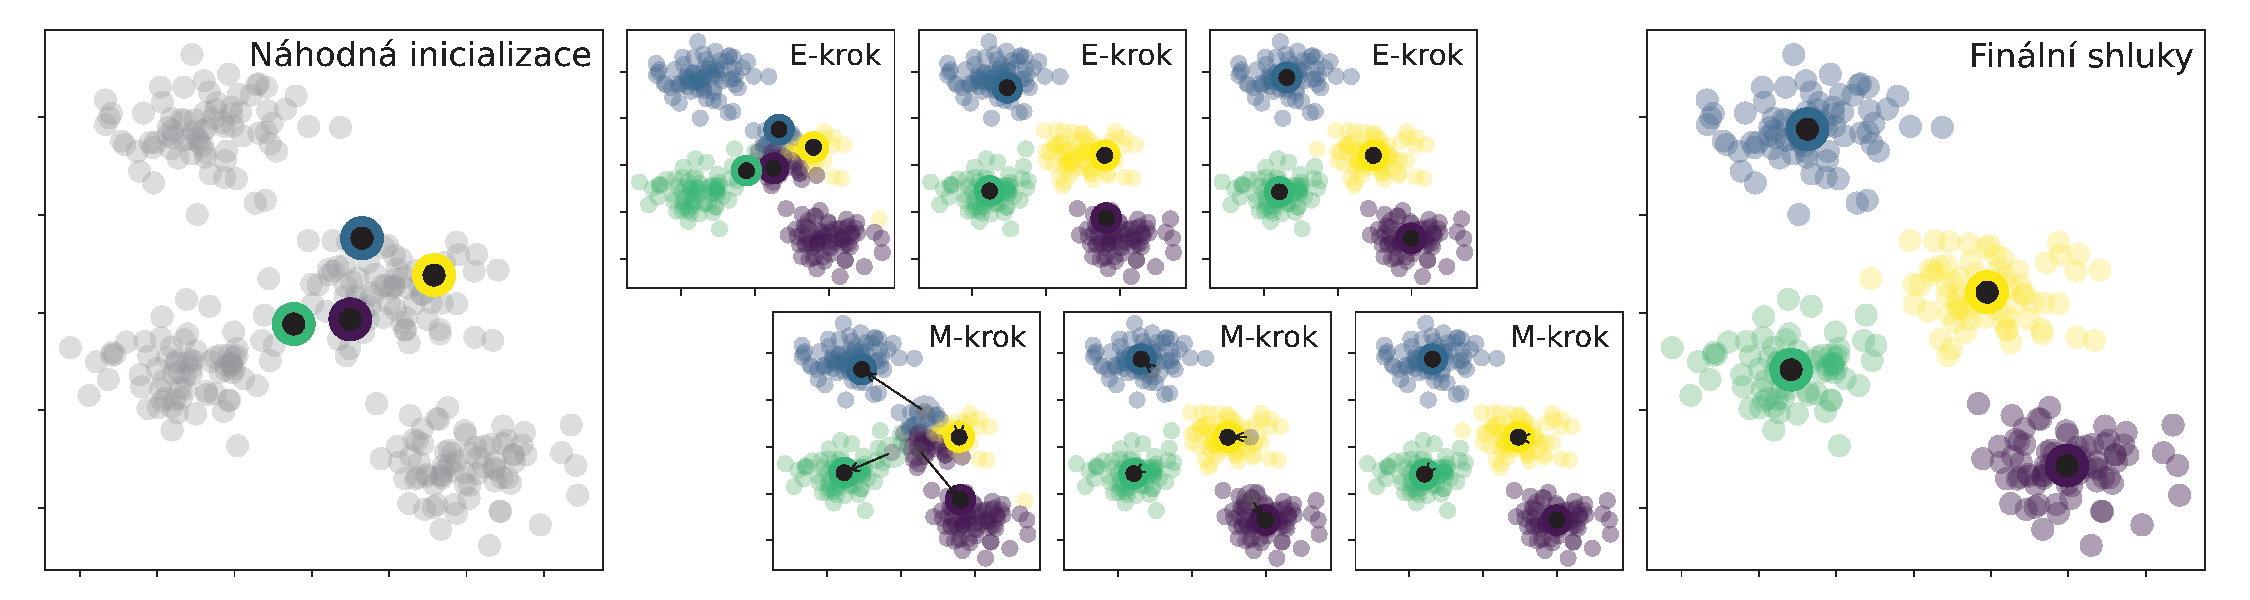
\includegraphics[width=1\linewidth]{img/pdfa-kmeans_example.pdf}
    \caption{Příklad průběhu algoritmu k-means. Černé kruhy značí centroidy, 
    barevné lemování slouží k jejich odlišení. Barva jednotlivých bodů
    značí náležení bodu do shluku centroidu s příslušnou barvou.}
    \label{fig:kmeans_example}
\end{figure}


\section{A-star}
\label{sec:a_star}
\emph{A-star} (A*) je algoritmus pro vyhledávání optimálních cest v kladně 
ohodnocených grafech. Jedná se o modifikaci Dijkstrova algoritmu s přidaným 
heuristickým prvkem.

Výpočet algoritmu je téměř totožný s Dijkstrovým algoritmem, od něhož se 
odlišuje ve výběru následujícího vrcholu pro otevření, který volí na základě
funkce $f(x) := g(x) + h(x)$. Funkce $g(x)$ zde označuje reálnou (nalezenou) 
vzdálenost od počátečního bodu do bodu $x$ (Dijkstrův algoritmus pracuje pouze 
s touto hodnotou). Funkce $h(x)$, pak značí heuristickou funkci odhadující 
vzdálenost vrcholu $x$ od požadovaného cílového vrcholu. Pokud je heuristická 
funkce vhodně zvolena, je možné znatelně omezit počet operací pro nalezení nejkratší
cesty mezi dvěma vrcholy v porovnání s Dijkstrovým algoritmem. 

Typicky je u heuristické funkce $h$ požadována tzv. \emph{přípustnost} 
(nenahodnocuje vzdálenost do cíle), či \emph{monotónost} 
(hodnota funkce $h$ roste po přechodu na další hranu), více
informací o tomto algoritmu popisuje \citet{russell2010artificial}.


\section{Související práce}
\label{sec:souvisejici_prace}

V této sekci si popíšeme několik souvisejících prací a stručně popíšeme 
jejich vlastnosti.


Simulátor SUMO\footnote{\url{https://www.eclipse.org/sumo/}} je velmi detailní
simulátor dopravy v rozsahu funkcionalit zdaleka přesahující naši implementaci.
V programu lze do jisté míry simulovat také elektromobily. Pro naše učely je
ale tento program velmi komplexní a práce s optimalizačními algoritmy
by tak byla neprakticky komplikovaná.

Simulátor City Flow\footnote{\url{https://cityflow.readthedocs.io/en/latest/index.html}}
se pyšní především výpočetní efektivitou\footnote{\url{https://cityflow.readthedocs.io/en/latest/introduction.html}}.
Bohužel nenabízí jednoduché uživatelské rozhraní pro rozšíření o metody
potřebné pro naši optimalizaci.

V práci \citet{kmeans_layout} je navržen simulátor dopravy pro následnou 
analýzu nově navrženého optimalizačního algoritmu rozmístění nabíjecích stanic
na území Japonska. Optimalizační algoritmus v práci se snaží minimalizovat 
počet vozidel, kterým se vybila baterie, pomocí posunů nabíjecích stanic směrem
k místům, kde se v minulosti vybila baterie vozidla. Návrh simulátoru naší práce
a optimalizační algoritmus s použití metody k-means jsou inspirovány zmíněnou
prací.

V práci \citet{niccolai2021optimization} je zkoumáno několik variant evolučních
algoritmů pro optimalizaci rozmístění nabíjecích stanic elektrických vozidel
ve městě Milán. V práci byl porovnáván také hladový přístup rozmísťující 
iterativně nabíjecí stanice na místa lokálních extrémů specificky zadefinované
ztrátové funkce. 

Práce \citet{zhu2016charging} se zabývá optimalizací rozmístění nabíjecích 
stanic v okolí města Peking užitím technik genetického algoritmu. V práci 
jsou porovnávány dvě varianty modelů popisující možné pozice nabíjecích stanic a
je v ní poukázáno, že správná volba modelu ovlivňuje kvalitu řešení optimalizace. 

V práci \citet{kinay2021full} je navžen simulátor pro rozvrhování pozic 
nabíjecích stanic. Problém je zde matematicky popsán. V práci jsou navrženy
dvě varianty optimalizací. Jedna minimalizující celkovou cenu rozmístění 
nabíjecích stanic s minimalizací odchylek od původní trasy, druhá optimalizuje
pozice stanic s ohledem na minimalizaci odchylek.
\chapter{Příprava mapy silniční sítě}
\label{chap:priprava_mapy}

Hlavní motivací pro vytvoření simulátoru dopravy je vytvoření uživatelsky
přívětivého prostředí pro práci s různými variantami rozmístění nabíjecích 
stanic na reálné dopravní síti. Je tedy více než žádoucí pracovat s reprezentací
reálné silniční sítě. K tomuto účelu používáme volně dostupné mapy formátu
\texttt{.osm.pbf} ze serveru 
Geofabric\footnote{\url{https://download.geofabrik.de/}}. 

V této kapitole popisujeme jakým způsobem lze zmíněné mapy upravit do formátu
požadovaného naším simulátorem a poukazujeme na důležité poznatky této problematiky. 
V našich experimentech pracujeme s reprezentací mapy 
České republiky\footnote{\url{https://download.geofabrik.de/europe/czech-republic.html}},
která je přiložena k práci v již požadovaném formátu simulátoru a pro správné spuštění
simulátoru tak postupy popsané v této kapitole nejsou nutné. 


\section{Extrakce dopravní sítě}
\label{sec:extrakce_site}

V této sekci popisujeme proces extrakce dopravní sítě z mapy formátu 
\texttt{.osm.pbf} do formátu požadovaného našim simulátorem a poukazujeme
na specifické aspekty námi zvolené mapy pro analýzu optimalizačních metod.


\subsection{Extrakce s pomocí nástroje Osmium}

Soubory formátu \texttt{.osm.pbf} obsahují mimo informace o dopravní síti,
také velké množství informací irelevantních pro funkci našeho simulátoru. 
Důsledkem této skutečnosti je několikanásobně vyšší množství dat pro 
zpracování, což mimo jiné vede k vyšší paměťové i časové náročnosti programu.
Je tak žádoucí všechny nepotřebné informace odstranit. K tomuto účelu
používáme nástroj \texttt{Osmium}\footnote{\url{https://osmcode.org/osmium-tool/}}.
S jehož pomocí jsme schopni z mapy vyextrahovat silniční síť a zároveň
vybrat pouze námi zvolené druhy silnic.

\subsubsection{Dodatek k výběru druhů silnic}
Mezi zvolené typy silnic, které náš simulátor rozeznává, patří 
dálnice, silnice pro motorová vozidla a silnice první třídy (v kontextu
dat se jedná o typy \texttt{motorway}, \texttt{trunk} a \texttt{primary}).
Silnice nižších tříd jsme zanedbali, neboť předpokládáme, že výše zmíněné 
silnice tvoří souvislý graf, případně, že jsou rozděleny do relativně nízkého 
počtu komponent souvislosti a dostatečně aproximují zkoumanou dopravní síť.
S ohledem na skutečnost, že v reálném případě je silniční síť v naprosté většině
případů souvislý graf, je žádoucí minimalizovat rozpad dopravní sítě na 
komponenty souvislosti. V našem případě je graf rozdělen do 75 komponent 
souvislosti, což se jeví jako poměrně vysoké číslo a vyvolává pochybnosti,
zda je naše volba typů silnic vhodná. Vysoký počet komponent si odůvodňujeme
výběrem mapy pokrývající pouze výřez reálné oblasti, což může vézt k rozpadu
silniční sítě na více komponent souvislosti především v hraničních oblastech.

Významným faktorem podněcujícím k eliminaci silnic nižší třídy je fakt, že
s klesající třídou silnic typicky několikanásobně roste jejich počet. Výsledný
graf je pak mnohonásobně hustší, což vede k vyšší výpočetní náročnosti celého
simulátoru, případně na méně výkonných strojích k nepoužitelnosti simulátoru
z časových i paměťových důvodů. V našem případě vzrostl počet hran grafu při
zahrnutí silnic 2. třídy asi pětinásobně. 

Předpokládáme, že neexistuje mnoho hustě osídleným oblastí v simulované oblasti,
které bychom takto vyloučili ze simulace. Jelikož předpokládáme, že hustěji
osídlené oblasti mají v blízkém okolí přístup k silnicím vyšších tříd. 
Nevýhodou tohoto přístupu je zanedbání realistické reprezentace sítě na úrovni
jednotlivých měst, či malých oblastí. Nemůžeme tak dostatečně realisticky 
simulovat například průjezdy vozidel křižovatkou, dopravní zácpy ve městech apod.
Zároveň jsme omezeni na cesty vozidel vedoucích pouze po silnicích vyšší třídy. 
Předpokládáme však že tato omezení nejsou s ohledem
na námi řešený problém nijak závažná, neboť nás zajímají především dálkové 
cesty, během nichž je častější potřeba řidiče použít nabíjecí stanici.


\subsubsection{Extrakce měst}

Pro dosažení co nejrealističtějších výsledků simulace je potřeba vhodně
generovat počáteční a cílové pozice vozidel. K tomuto účelu nám slouží informace
o pozicích a počtu obyvatel osídlených oblastí na mapě. 
Pro získání těchto informací nám znovu poslouží nástroj \texttt{Osmium}. 
S jeho pomocí získáváme informace o městech (oblasti označené jako \texttt{city}
nebo \texttt{town}). 

Vynechali jsme menší osídlené oblasti, jelikož předpokládáme, že
počet výjezdů a cílů cesty je v této oblastí zanedbatelný. Navíc je počet
menších celků vysoký a jejich zahrnutí by vyžadovalo více výpočetního výkonu.


\subsection{Příprava dat pomocným skriptem}

Postupy popsanými výše jsme získané informace zásadně zredukovali. Veškerá 
vyfiltrovaná data jsou ale stále ve formátu \texttt{osm.pbf}, který musíme 
vhodným způsobem zpracovat a odstranit nepotřebné informace o silnicích
a obytných oblastech. K tomuto účelu jsme využili knihovny programovacího
jazyka Python \texttt{Pyrosm}\footnote{\url{https://pyrosm.readthedocs.io/en/latest/}}.
A naimplementovali program v jazyce Python, jenž načte data ze souborů ve formátu
\texttt{osm.pbf} a náležitě je upraví do podoby vstupních souborů našeho 
simulátoru dopravy. Podrobnější informace k přípravě dat i veškeré programy 
jsou dodány v příloze v adresáři \texttt{map\_processing}. 


\section{Dodatek k volbě programovacího jazyka a nutnosti předpřípravy dat}

Pro správné fungování simulátoru není práce s nástroji popsanými v sekci (\cref{sec:extrakce_site}).
nutná (je například možné pracovat s ručně připravenou reprezentací
dopravní sítě a nerešit jakoukoli přípravu dat z reálných map).

Reprezentace mapy ve formátu \texttt{osm.pbf} je obecně velmi rozšířená, což má za 
následek existenci početné skupiny knihoven (především v jazyce Python), jež umí
s těmito soubory pracovat a vhodným způsobem je zpracovávat. Zároveň existuje 
řada knihoven programovacího jazyka Python, které nabízejí širokou
škálu funkcionalit pro práci s grafy a grafovými algoritmy. 
Může nám tedy připadat kontraproduktivní pracovat s několika různými 
nástroji pro předpřípravu dat a pracovat s více programovacími jazyky, 
když lze většinu funkcionalit pokrýt programem napsaným v jazyce Python s 
využitím vhodných knihoven. 
Původním cílem práce bylo zvolit tento přístup. Během práce na simulátoru 
jsme však narazili na vysokou paměťovou i časovou náročnost tohoto postupu
a upustili jsme od něj.  
Na základě těchto skutečností jsme se nakonec rozhodli v jazyce Python 
pouze předzpracovat data a zbytek simulátoru naimplementovat v 
jazyce C++ s využitím knihovny \texttt{boost}\footnote{\url{https://www.boost.org/}}.

\chapter{Popis simulátoru}
\label{chap:popis_simulatoru}

V této kapitole definujeme řadu důležitých pojmů pro správný popis simulátoru
a dále popisujeme veškeré vlastnosti a funkcionality simulátoru.

Hlavní cílem návrhu simulátoru je uživatelská přívětivost v rámci analýzy
různých variant optimalizačních algoritmů. S ohledem na námi řešený problém je 
kladen důraz především na rozšířitelnost programu o nové optimalizační techniky
a snadnou nastavitelnost parametrů úzce souvisejících
s vlastnostmi nabíjecích stanic, mezi něž patří například počet nabíjecích stanic, 
rozmístění stanic, počet nabíjecích slotů na stanicích a podobně.

\section{Poznámka ke značení a definicím}
V následujícím textu definujeme řadu objektů simulace, jenž jsou často reprezentovány
uspořádanou množinou veličin. Často budeme potřebovat specifikovat jednotlivé 
složky těchto objektů. Pro zjednodušení notace, tak budeme zapisovat parametry
ve formátu \texttt{objekt.jméno\_parametru}. 

Tedy pokud například definujeme objekt $o$ jako uspořádanou množinu $(x, y, z)$.
Pak parametr $y$ objektu $o$ zapisujeme ve formátu $o.y$.

Dále je potřeba zmínit, že některé definice uvedené v následujícím textu, jsou
zjednodušeny a jejich zápis nemusí být matematicky naprosto přesný. 
Jsou například vynechány nějaké předpoklady z definic, které zřejmě vyplývají z 
textu. K tomuto kroku bylo přistoupeno pod snahou zpřehlednit jednotlivé definice.


\section{Předpoklady návrhu modelu}
\label{sec:predpoklady_navrhu}
S ohledem na výpočetní efektivitu simulátoru a uživatelskou přívětivost je potřeba
náležitě zjednodušit simulovaný model.

Dopravní síť reprezentujeme vhodným grafem rozšířeným o potřebné parametry. Simulátor je
navržen pro simulaci dopravních sítí pokrývající větší územní celky, které jsou 
rozlohou a hustotou sítě srovnatelné s dopravní sítí České republiky. Z tohoto
důvodu není zaručeno vhodné chování simulace na dopravních sítích s výrazně odlišnými
vlastnostmi.

Při volbě velikosti simulované oblasti jsme předpokládali, že většina majitelů
vozidel má možnost dobíjet své vozy v počáteční a cílové destinaci (např. mají
nabíjecí sloty v místě bydliště, či na pracovišti). Pro cesty na krátké vzdálenosti
tak budou schopni dobít své automobily na dostatečnou hladinu baterie a během cesty
nebude potřeba použít nabíjecí stanici. 

Na základě tohoto předpokladu je kladen důraz především na realistické simulování
dálkových tras vozidel. V zájmu výpočetní efektivity simulátoru a zkoumaného problému
opomíjíme většinu cest na krátkou vzdálenost a naopak nadhodnocujeme počet dálkových
tras vozidel. V simulátoru je nastavitelná střední hodnota vzdálenosti trasy, čímž
můžeme míru tohoto předpokladu náležitě regulovat.

Důsledkem zjednodušení je v simulaci zanedbána část vlastností reálné 
dopravní sítě. Například hustota provozu či skutečnost, že v reálném 
případě budou nabíjecí stanici využívat také řidiči jedoucí na krátké 
vzdálenosti tak nebude v simulaci dostatečně zahrnuta.

Protože je v reálném případě dopravní síť značně komplexní (především na 
úrovni silnic nižší třídy), je potřeba síť řádně zjednodušit. Tato problematika
je podrobněji popsána v kapitole o přípravě mapy viz. \cref{chap:priprava_mapy}.


\section{Dopravní síť}
\label{sec:dopravni_sit}

Řada myšlenek použitých pro definici modelu silniční sítě je inspirována 
návrhem modelu v práci \citet{kmeans_layout}.

Dopravní síť je v zájmu efektivity a jednoduchosti simulace reprezentována
vhodným grafem. K popisu grafu potřebujeme nejprve zadefinovat několik 
pomocných pojmů a objektů simulátoru.

Prvním pojmem je \emph{křižovatka}, jež zastupuje podmnožinu vrcholů v 
grafu silniční sítě, které reprezentují křižovatky v reálné silniční síti.

\begin{defn}[Křižovatka]\label{def:krizovatka}
    \emph{Křižovatka} je uspořádaná čtveřice $(n, c, m, d)$, kde:
    \begin{itemize}
        \item $n \in \mathbb{N}_0$ - identifikátor
        \item $c \in \mathbb{R}^2$ - zeměpisné souřadnice (viz. \cref{sect:zem_souradnice})
        \item $m \in \mathbb{N}_0$  - identifikátor nejbližšího města od křižovatky
        \item $d \in \mathbb{R}$ - vzdálenost vrcholu od středu města s 
        identifikátorem $m$
    \end{itemize}
\end{defn} 

Dále definujme \emph{typy silnice} používané simulátorem, s jejichž pomocí můžeme v
simulaci dopravy rozlišovat mezi různými kapacitami jednotlivých úseků dopravní sítě
(např. dálnice typicky efektivněji pokryjí hustý provoz než silnice 1. třídy).

\begin{defn}[Množina typů silnice]\label{def:mnoz_typu_silnice}
    \emph{Množina typů silnice} je množina $\{m, t, p, o\}$ všech typů 
    silnice používaných v simulaci dopravní sítě, kde:
    \begin{itemize}
        \item $m$ - dálnice
        \item $t$ - silnice pro motorová vozidla
        \item $p$ - silnice 1. třídy
        \item $o$ - ostatní typy silnic
    \end{itemize}
\end{defn}

\emph{Segmenty silnic} reprezentují vybrané body v silniční síti. A slouží jako
vrcholy grafu.

\begin{defn}[Segment silnice]\label{def:segment_silnice}
    \emph{Segment silnice} je uspořádaná dvojice $(n, b)$, kde:
    \begin{itemize}
        \item $n \in \mathbb{N}_0$ - identifikátor segmentu (určuje přesnou pozici)
        \item $b \in [0, 1]$ - průměrná hladina baterie vozidel v místě segmentu
    \end{itemize}
\end{defn}

\emph{Silnice} reprezentuje část silniční sítě mezi 2 křižovatkami, jenž neprochází
žádnou křižovatkou. Tento objekt shlukuje všechny segmenty silnice mezi dvojicemi
křižovatek.

\begin{defn}[Silnice]\label{def:silnice}
    Nechť $K$ značí množinu všech křižovatek v silniční síti a
    $T$ značí množinu typů silnic. Zároveň předpokládejme, že $k_1 < k_2$,  
    
    Pak \emph{silnice nad množinou křižovatek $K$} je uspořádaná
    pětice $(k_1, k_2, d, t, S)$, kde:
    \begin{itemize}
        \item $k_1, k_2 \in K$ - křižovatky na koncích silnice 
        \item $d \in \mathbb{R}^+$ - délka segmentu silnice
        \item $t \in T$ - typ
        \item $S$ - množina segmentů silnice, pro kterou je splněna podmínka: 
        $$(\forall{s, r} \in \mathbb{N}; r < s)(s \in S \implies r \in S)$$
    \end{itemize}
\end{defn}

Nyní již můžeme zadefinovat \emph{graf dopravní sítě}, s nímž pracujeme v naší simulaci
dopravy.

\begin{defn}[Graf dopravní sítě]\label{def:graf_site}
    Mějme množinu křižovatek $K$, množinu silnic $R$ nad množinou 
    křižovatek $K$ a $d \in \mathbb{R}$, pro které jsou splněny podmínky:
    \begin{enumerate}
        \item $$(\forall r_1, r_2 \in R; r_1 \neq r_2)\left(|r_1.S \cap r_2.S| \leq 1\right)$$
        \item $$(\forall r_1, r_2 \in R)\left(\{r_1.k_1, r_1.k_2\} 
            \cap \{r_2.k_1, r_2.k_2\} = \emptyset 
            \implies r_1.S \cap r_2.S = \emptyset \right)$$
        \item $$(\forall r \in R)(r.d = d)$$
    \end{enumerate}
    
    Definujme množinu segmentů všech silnic z $R$:
        $$V = \bigcup_{r \in R} r.S$$
    Následně definujme množinu sousedních dvojic segmentů silnice $r \in R$ jako:
        $$E_r = \{(s_1, s_2) \in (r.S)^2; |s_1.n - s_2.n| = 1\}$$
    A množinu sousedních dvojic segmentů všech silnic z $R$ jako:
        $$E = \bigcup_{r \in R} E_r$$

    Pak \emph{graf dopravní sítě} $G=(V, E)$ je uniformně ohodnocený souvislý 
    graf s vrcholy $V$ a hranami $E$ délky $d$.
\end{defn}

\section{Objekty dopravní sítě}

\subsection{Segmenty}
Segmenty silnice z \cref{def:segment_silnice} jsou nejmenší stavební jednotkou
celého simulátoru. Reprezentují vrcholy grafu silniční sítě a slouží k 
diskretizaci reálné silniční sítě, která je s jejich pomocí rozdělena 
na uniformně dlouhé úseky. Uchovává informaci o průměrné hladině baterie
v jednotlivých usecích dopravní sítě, která je využívána v optimalizaci.


\subsection{Křižovatky}
Křižovatky z \cref{def:krizovatka} zastupují podmnožinu vrcholů grafů
sítě, stupně vyššího než 2. Společně s městy se jedná o jediné objekty 
simulátoru, jenž si uchovávají zeměpisnou polohu v reálné dopravní síti.

Za pomocí těchto objektů jsou v simulátoru významným způsobem optimalizovány
algoritmy pro grafové hledání optimální cesty. Jsou používány k redukci vrcholů
a hran prohledávaného grafu, k heuristickému prohledávání stavového prostoru
při hledání nejkratších cest, či vhodných nabíjecích stanic. Jsou také hojně
používány v optimalizačních algoritmech pro rozmístění nabíjecích stanic.


\subsection{Silnice}

Silnice z \cref{def:silnice} sdružují podmnožinu hran grafu ležící mezi
2 křižovatkami a neprocházející jinou křižovatkou. Jsou potřebné pro 
zadefinování hran grafu simulátoru. Uchovávají informaci
o typu silnice, jsou používány pro hledání nejkratší cesty v grafu a jsou 
používány k simulování hustoty provozu v různých částech dopravní sítě.

V simulátoru předpokládáme, že délky všech silnic dopravní sítě jsou 
dělitelné délkou segmentu. To však v reálném případě typicky nenastane. V 
popisu reálné silniční sítě pracujeme pouze s přibližnou délkou jednotlivých
silnic. Tato skutečnost však výrazně neovlivňuje námi požadované vlastnosti
simulace.

\subsubsection{Hustota provozu}
Silnice je používána pro simulování hustoty provozu v jednotlivých úsecích dopravní
sítě. V simulátoru je zaimplementována jednoduchá logika pracující s hustotou
provozu v závislosti na typu (viz. \cref{def:mnoz_typu_silnice}) a délce 
silnice.

Princip simulování hustoty provozu je založen myšlence \emph{kapacity silnice}.

\begin{defn}[Kapacita silnice]\label{def:kapacita_silnice}
    Mějme $d$ délku hran grafu dopravní sítě $G$ z \cref{def:graf_site}.
    Nechť $R$ je množina silnic $G$. Dále $f:T \to \mathbb{R}$, kde $T$ je 
    množina všech typů silnic z \cref{def:silnice} a $\alpha, \beta \in \mathbb{R}$.

    \emph{Kapacita silnice} je funkce $c:R \to \mathbb{R}^+$, definována jako:
        $$c(r) := \alpha \cdot f(r.t) + \beta \cdot d \cdot |r.S|$$
\end{defn}

V simulátoru byly hodnoty $\alpha, \beta$ zvoleny na základě empirické volby. 
Simulování hustoty provozu je pak odvozeno od aktuálního počtu vozidel na 
silnici. Pomocí jednoduché funkce \emph{relativní délky silnice}.
 
\begin{defn}[Relativní délka silnice]\label{def:relativni_delka_silnice}
    Mějme $d$ délku hran grafu dopravní sítě $G$. Silnici $r$ grafu $G$,
    jejíž kapacita je $c_r \in \mathbb{R}^+$ a 
    nechť $n_r \in \mathbb{N}_0$ je aktuální počet vozidel na 
    silnici $r$. Dále funkce zpoždění vozidla $f:\mathbb{R} \to \mathbb{R}^+$.

    \emph{Relativní délka silnice} $r$ je definována, jako 
    $t_r:\mathbb{R}^+ \times \mathbb{N}_0 \to \mathbb{R}^+$, kde:
    $$
        t_{r}(n_r) =
          \begin{cases}
            |r.S| & pro\ n_r \leq c_r \\
            |r.S| \cdot f(n_r - c_r) & pro\ n_r > c_r
          \end{cases}       
    $$
\end{defn}

Doba průjezdu vozidla po silnici se pak vypočítá jako doba potřebná pro ujetí
vzdálenosti $d$, která je rovna relativní délce silnice, vozidlem s pevně
zvolenou průměrnou rychlostí $v$ (danou parametry simulátoru). Simulátor 
vždy aktualizuje hodnotu relativní délky silnice po změně počtu vozidel 
na silnici.


\subsection{Města}
Důležitým prvkem simulátoru je zakomponování vlivu zalidnění simulovaných oblastí.
K tomuto účelu nám slouží objekt \emph{město}.

\begin{defn}[Město]\label{def:mesto}
    \emph{Město} je uspořádaná trojice $(n, c, p)$, kde:
    \begin{itemize}
        \item $n \in \mathbb{N}_0$ - identifikátor
        \item $c \in \mathbb{R}^2$ - zeměpisné souřadnice centra města 
        (viz. \cref{sect:zem_souradnice})
        \item $p \in \mathbb{N}_0$ - počet obyvatel města
    \end{itemize}
\end{defn}

Každému městu náleží příslušná množina křižovatek definována jako:

\begin{defn}[Množina křižovatek města]\label{def:krizovatky_mesta}
    Mějme město $m$ v simulátoru a množinu všech křižovatek $K$ grafu $G$,
    pak \emph{množina křižovatek města} je:
    $$K_m = \{k \in K| k.m = m.n\}$$ 
\end{defn}

Koncept měst je důležitý pro realističtější generování počátečních
a koncových pozic vozidel v simulaci. Slouží také pro heuristický
výběr vhodné nabíjecí stanice pro nabití vozu.


\subsection{Nabíjecí stanice}
\emph{Nabíjecí stanice} jsou vzhledem ke zkoumanému problému důležitým 
prvkem simulátoru.

\begin{defn}[Nabíjecí stanice]\label{def:nabijeci_stanice}
    \emph{Nabíjecí stanice} v grafu dopravní sítě $G=(V, E)$ je uspořádaná 
    čtveřice $(n, m, v, c)$, kde:
    \begin{itemize}
        \item $n \in \mathbb{N}_0$ - identifikátor
        \item $m \in \mathbb{N}_0$ - identifikátor nejbližšího města od stanice
        \item $v \in V$ - pozice stanice (vrchol v grafu dopravní sítě)
        \item $c \in \mathbb{N}$ - kapacita stanice (počet zákazníků, 
        jež stanice pokryje najednou)
    \end{itemize}
\end{defn}

Informace o nejbližším městě je důležitá především pro heuristickou volbu 
nabíjecí stanice vozidlem v simulaci. V simulátoru je uchovávána informace
o aktuálním vytížení stanice a o vozidlech čekajících na volný nabíjecí slot pro 
simulování čekání automobilů ve frontě. Simulátor si pro každou nabíjecí 
stanici pamatuje průměrnou hladinu baterie vozidel při příjezdu do stanice,
pro použití v optimalizačních algoritmech. 
V návrhu simulátoru předpokládáme, že zákazníci stanice dobíjejí své vozidlo 
na plnou kapacitu baterie. Návrh simulátoru však umožňuje rozšíření o 
nabíjení pouze na zvolenou hladinu baterie bez významnějších zásahů do původní
implementace.


\section{Vozidla}
\label{sec:vozidla}

\emph{Vozidla} jsou nejdůležitějším prvkem simulace. Jednotlivá vozidla jsou 
simulátorem spravována samostatně. Každému vozidlu je při generování přiřazena
počáteční a cílová pozice a počáteční hladina baterie.


\subsection{Generování vozidel}
\label{subsec:generovani_vozidel}

Vozidla jsou v simulaci generována, aby co nejlépe aproximovala reálný provoz
vozidel. Doba čekání mezi výjezdy vozidel je náhodně generována z exponenciální
distribuce s nastavitelnými parametry. Počáteční hladina baterie vozidla je 
vygenerována z normálního rozdělení s pevně zvolenými parametry. Definujeme
také horní a dolní hranici hladiny počáteční baterie. Pokud vygenerovaná
hladina překračuje jednu z těchto hranic, pak je nahrazena hodnotou
překročené hranice.
Tento krok slouží jako ochrana pro vygenerování hladiny baterie pouze
v rozmezí $[0, 1]$.


Počáteční i cílová pozice vozidla je generována několikafázově z kombinace 
více náhodných distribucí. 

Při generování pozice výjezdu je nejprve generováno město $m_1$ výjezdu s 
pravděpodobností úměrnou jeho počtu obyvatel (čím více obyvatel, tím je 
výjezd vozidla pravděpodobnější). Tedy:

\begin{defn}[Pravděpodobnost výjezdu z města]\label{def:pravdepodobnost_mesta}
    Zvolme množinu $M$ všech měst v simulátoru. Pak 
    \emph{pravděpodobnost výjezdu} vozidla z města $m \in M$, je rovna:
        $$p_m = \frac{m.p}{\sum_{m_i \in M} m_i.p}$$
\end{defn}

Po vygenerování počátečního města $m_1$ je uniformně náhodně zvolena 
křižovatka $k_1$ z množiny křižovatek města $m_1$ 
(viz. \cref{def:krizovatky_mesta}). Následně je uniformně náhodně vybrána
silnice $r_1$ napojená na křižovatku $k_1$. Neboli silnice $r_1$, pro kterou
platí $ k_1 \in \{r_1.k_1, r_1.k_2\}$. Nakonec je uniformně náhodně zvolen
segment $v_1$ (vrchol grafu silniční sítě) silnice $r_1$, který již jednoznačně
popisuje pozici výjezdu vozidla. 

Generování cílové pozice vozidel je realizováno podobně s rozdílem generování 
koncového města. Při náhodném výběru koncového města je pravděpodobnost
výběru města ovlivněna počtem obyvatel města a vzdáleností od počátečního města.

Proces generování cílového města probíhá následovně. Nejprve je spočítána 
pravděpodobnost výjezdu vozidla pro všechna města v simulátoru 
(viz. \cref{def:pravdepodobnost_mesta}). Dále je pro počáteční město $m_1$
a každé město $m_i \in M$ simulátoru vypočítána jejich geografická vzdálenost
(viz. \cref{sect:zem_souradnice}), kterou označíme jako $d_{1,i}$. 
Následně pro všechna města $m_i \in M$ vypočítáme pravděpodobnost vzdálenosti $d_{1,i}$,
kterou si označíme $p_{1,i}$. Pravděpodobnost vzdálenosti $p_{1,i}$ vypočítáme
s pomocí nastavitelné exponenciální distribuce popisující vzdálenost cílové
pozice od počáteční pozice. Pravděpodobnost cílového města $m_2 \in M$
vůči počátečnímu městu $m_1 \in M$ spočítáme následovně:

\begin{defn}[Pravděpodobnost cílového města]\label{def:pravdepodobnost_ciloveho_mesta}
    Mějme $\alpha \in \mathbb{R}^+$ a počáteční město $m_1 \in M$. Označme vzdálenost 
    města $m_1$ od města $m_2 \in M$ jako $d_{m_1,m_2} \in \mathbb{R}$. 
    Označme pravděpodobnost
    výjezdu z města $m_2$ jako $p_{m_2}$ a pravděpodobnost vzdálenosti $d_{m_1,m_2}$ jako
    $p_{m_1,m_2}$, kterou dostaneme z námi zvolené exponenciální distribuce 
    (stejná notace platí pro libovolné město $m_i \in M$).
    Pak pravděpodobnost $p_{m_1,m_{2_{final}}}$, že město $m_2$ je cílovým městem
    vozidla s počátkem ve městě $m_1$ je rovna:
        $$p_{m_1,m_{2_{final}}} = 
            \frac{p_{m_2} + \alpha \cdot p_{m_1,m_2}}
            {\sum_{m_i \in M} p_{m_i} + \alpha \cdot p_{m_1,m_i}}$$
\end{defn}

Cílové město $m_2 \in M$ vygenerujeme z distribuce měst dané pravděpodobnostmi
cílového města vůči počátečními městu $m_1$ (viz. \cref{def:pravdepodobnost_ciloveho_mesta}).
Proces generování přesné cílové pozice ve městě $m_2$ je totožný s procesem 
generování přesné počáteční pozice ve zvoleném městě $m \in M$.

\begin{algorithm}
\begin{algorithmic}
\Function{Generování náhodné pozice}{$m$ - město}
    \State Uniformně náhodně vygeneruj křižovatku $k$ ve městě $m$.
    \State Uniformně náhodně vygeneruj silnici $r$ napojenou na křižovatku $k$.
    \State Uniformně náhodně vygeneruj segment $v$ na silnici $r$.
    \State \Return $v$
\EndFunction
\end{algorithmic}
\caption{Postup při náhodném generování pozice ve městě (vrcholu v grafu).}
\label{alg:generovani_pozice_ve_meste}
\end{algorithm}


\begin{algorithm}
\begin{algorithmic}
\Function{Generování vozidla}{}
    \State Z normálního rozdělení vygeneruj počáteční hladinu baterie $b$.
    \State V závislosti na počtu obyvatel náhodně vygeneruj počáteční město $m_1$.
    \State $v_1 \gets$ \Call{Generování náhodné pozice}{$m_1$}
    \State V závislosti na počtu obyvatel a vzdálenosti of města $m_1$ náhodně vygeneruj
    koncové město $m_2$
    \State $v_2 \gets$ \Call{Generování náhodné pozice}{$m_2$} 
    \State Z exponenciální distribuce vygeneruj čas $t$ čekání na výjezd vozidla.
    \State $vehicle \gets$ vozidlo s počáteční hladinou baterie $b$, 
    počátečním vrcholem $v_1$ a cílovým vrcholem $v_2$.
    \State \Return $vehicle$, $t$ \Comment vygenerovené vozidlo a čas čekání na jeho výjezd.

\EndFunction
\end{algorithmic}
\caption{Pseudokód procesu generování nového vozidla v simulaci.}
\label{alg:generovani_vozidla}
\end{algorithm}


\subsection{Hledání trasy vozidla}
\label{subsec:hledani_trasy}

Po vygenerování vozidla musíme v simulátoru vyřešit také otázku naplánování
trasy vozidla, které je realizováno algoritmem A-star (viz. \cref{sec:a_star}),
který jako heuristickou funkci volí zeměpisnou vzdálenost 
(viz. \cref{sect:zem_souradnice}) mezi křižovatkami.

S ohledem na efektivitu výpočtu pracujeme v simulaci při hledání cesty
se \emph{zjednodušeným grafem dopravní sítě} vůči počátečnímu vrcholu 
$v_1$ a cílovému vrcholu $v_2$.

\begin{defn}[Zjednodušený graf dopravní sítě]\label{def:zjednodusena_dopravni_site}
    Mějme graf dopravní sítě $G=(V, E)$ (viz. \cref{def:graf_site}) s množinou
    křižovatek $K$ a množinou silnic v síti $R$. Zvolme počáteční $v_1 \in V$ 
    a koncový vrchol $v_2 \in V$ a silnice $r_1 \in R$, resp. $r_2 \in R$, 
    t.ž. $v_1 \in r_1.S$, resp. $v_2 \in r_2.S$. 

    \emph{Zjednodušený graf dopravní sítě} vůči počátečnímu vrcholu $v_1$ a koncovému
    vrcholu $v_2$ je graf $H=(V', E')$, kde:
    \begin{itemize}
        \item $V' = K \cup r_1.S \cup r_2.S$
        \item $E' = (R \setminus \{r_1, r_2\}) \cup \{$hrany na silnicích $r_1$ a $r_2\}$
    \end{itemize}
\end{defn}

Zjednodušený graf dopravní sítě vůči počátečnímu vrcholu $v_1$ a cílovému vrcholu $v_2$
(viz. \cref{def:zjednodusena_dopravni_site}), je tedy graf, jehož vrcholy jsou křižovatky a
hrany jsou silnice, s vyjímkou počáteční a koncové silnice, jejichž reprezentace je
ponechána z původní \cref{def:graf_site} grafu dopravní sítě.

Postup plánování trasy vozidla je pak následující. Zvolíme vhodný zjednodušený graf dopravní
sítě a hrany grafu ohodnotíme relativní délkou silnice 
(viz. \cref{def:relativni_delka_silnice}), v případě počáteční a koncové silnice tuto
hodnotu náležitě rozdělíme mezi jednotlivé hrany na silnici. Následně na tomto grafu 
spustíme algoritmus A-star pro nalezení nejkratší cesty mezi vrcholy $v_1$ a $v_2$ s
ohledem na aktuální provoz v dopravní síti.

Algoritmus A-star používá jako heuristickou funkci zeměpisnou vzdálenost křižovatek. 
Neumíme však efektivně vypočítat tuto vzdálenost pro segmenty 
(viz. \cref{def:segment_silnice}). Při hledání nejkratší cesty se tedy omezujeme
pouze na hledání cest mezi nejbližšími křižovatkami počátečního a koncového vrcholu.
Výslednou cestu následně dostaneme řádným rozšířením cesty z počátečního a koncového
vrcholu do jejich nejbližších křižovatek. Vyjímkou je cesta uvnitř jedné silnice, kterou
nalezneme triviálně.

Vzhledem k výpočetní náročnosti hledání optimální cesty vozidla, hledáme tuto cestu
pouze při vygenerování vozidla, či ve speciálních případech, jako je například
plánování cesty na nabíjecí stanici, nebo cesty z nabíjecí stanice.


\subsection{Zajíždění na nabíjecí stanici}
\label{subsec:zajizdeni_na_nabijecku}

Speciální situace nastává v moment, kdy vozidlo potřebuje navštívit nabíjecí stanici.
V tomto případě je naplánována cesta z počáteční pozice do heuristicky zvolené
nabíjecí stanice postupem popsaným v části \cref{subsec:hledani_trasy}.
Po řádném nabití vozidla je pak stejným způsobem nalezena cesta ze stanice do
cílové pozice.

\subsubsection{Rozhodnutí o zajetí na nabíjecí stanici}

Každé vozidlo má možnost na základě aktuální hladiny baterie aktualizovat 
svou trasu tak, aby směřovala k nejbližší nabíjecí stanici. 
Z důvodu výpočetní náročnosti přepočítání trasy, může ale každé vozidlo
využít této možnosti pouze jednou. Po zajetí vozidla na nabíjecí stanici je mu
však tato možnost znovu přidělena.

Jelikož každé vozidlo může pozměnit svou trasu pouze jednou, je důležité zvolit
vhodný okamžik přeplánování trasy. Tento okamžik naplánujeme pomocí vhodně 
nastavitelného normálního rozdělení, ze kterého vygenerujeme hladinu baterie,
při které se v budoucnu rozhodneme zda zamíříme na nabíjecí stanici, či ne.

Volby okamžiku rozhodování s pomocí normálního rozdělení je motivován následujícími
myšlenkami. Nechceme vyrazit ani plánovat cestu na nabíjecí stanici moc brzy, neboť se 
může v průběhu cesty podstatně změnit hustota provozu a naplánovaná cesta
tedy nebude optimální. Zároveň je cesta na nabíjecí stanici při dostatečně vysoké 
hladině baterie zbytečná z důvodu malé kapacity baterie, kterou je možno doplnit.
Naopak v případě velmi nízké hladiny baterie, při níž aktualizujeme cestu, můžeme
narazit na problém, že vozidlo nedojede na nabíjecí stanici před úplným vybitím baterie.

Zda vozidlo v moment aktualizace cesty vyrazí na nabíjecí stanici, rozhodneme
na základě očekávané hladiny baterie vozidla v cílové destinaci, kterou vypočítáme
z aktuální hustoty provozu a spotřeby vozidla. V simulátoru je nastavitelná 
nejnižší očekávaná cílová hladina baterie, pro kterou vozidlo ještě nemění svou trasu,
tak aby směřovalo na nabíjecí stanici.


\subsubsection{Výběr nabíjecí stanice}

Vozidlo se musí v okamžiku rozhodnutí vyrazit na nabíjecí stanici rozhodnout,
kterou stanici zvolit. Toto rozhodnutí je realizováno heuristicky. 

Postup výběru stanice probíhá následovně. Pro každé město (viz. \cref{def:mesto})
je na začátku simulace nalezen námi zvolený počet očekávaných nejbližších 
nabíjecích stanic. Množinu těchto stanic pro libovolné město $m$ označíme 
jako $C_m$. 

Postup heuristického výběru nejbližších stanic města je následující. Pro každou stanici
$c$ zvolíme její nejbližší křižovatku $k$ (viz. \cref{def:krizovatka}) a město $m_k$,
do nějž křižovatka $k$ náleží (viz. \cref{def:krizovatky_mesta}). 
Vzdálenost stanice $c$ od libovolného města $m$ pak spočítáme jako součet $k.d$ a
zeměpisné vzdálenosti (viz. \cref{sect:zem_souradnice}) měst $m$ a $m_k$.

Následně pak v závislosti na městu $m$, kterému náleží křižovatka $k$,
která je nejblíže od aktuální pozice vozidla, zvolíme kandidáty na vhodné 
nabíjecí stanice pro zvolené vozidlo. Tito kandidáti jsou právě stanice 
$C_m$. Pro každého kandidáta $c \in C_m$ následně vypočítáme s pomocí relativních délek 
silnic (viz. \cref{def:relativni_delka_silnice}) očekávanou dobu cesty 
(délka cesty v grafu relativních délek) $d_c$ vedoucí z aktuální pozice přes
nabíjecí stanici $c$ do cílové pozice.
Zvolená nabíjecí stanice $c_{min} \in C_m$, je taková, 
že $d_{c_{min}}$ je nejmenší ze všech stanic z $C_m$.

\begin{algorithm}
\begin{algorithmic}
\Function{Výběr nabíjecí stanice}{\newline$v_{start}$ - aktuální pozice vozidla,\newline
    $v_{end}$ - cílová pozice vozidla,\newline
    $C_{closest}$ - množina množin nejbližších stanic každého města}
    \State $k \gets$ Nejbližší křižovatka od $v_{start}$.
    \State $C_{closest_m} \gets$ Množina z $C_{closest}$ náležící městu s ID $k.m$
    \State $d_{min} \gets 0$ \Comment Nejkratší očekávaná doba cesty.
    \State $c_{min}$ \Comment Aktuálně nejlepší stanice pro výběr. 
    \ForAll{$c \in C_{closest_m}$}
        \State $d_{in} \gets$ \Call{A-star}{$v_{start}$, $c.v$} 
            \Comment Očekávaná doba cesty do stanice.
        \State $d_{out} \gets$ \Call{A-star}{$c.v$, $v_{end}$}
            \Comment Očekávaná doba cesty ze stanice do cíle.
        \If{$d_{in} + d_{out} < d_{min}$ nebo $c_{min}$ není definováno}
            \State $c_{min} \gets c$ \Comment Aktualizace nejlepší stanice.
            \State $d_{min} \gets d_{in} + d_{out}$
        \EndIf
    \EndFor
    \State \Return c \Comment Předej vybranou nabíjecí stanici.
\EndFunction
\end{algorithmic}
\caption{Proces výběru nabíjecí stanice vozidlem.}
\label{alg:vyber_stanice}
\end{algorithm}

Tento zjednodušený přístup hledání vhodné nabíjecí stanice podstatně zefektivňuje
simulaci. Neboť výpočetně nejnáročnější operací celé simulace je hledání nejkratších
cest v grafu. Omezením výběru stanic rychlost simulace výrazně vzroste. 


\subsubsection{Nakládání s vybitými vozidly}

Simulátor musí řešit také případy, kdy se vozidlům vybije baterie a nemůžou 
dojet do cíle. V takovém případě je vozidlo vyřazeno ze simulace a dále již nijak
neovlivňuje simulaci. Veškeré informace o vozidlech s vybitými bateriemi jsou
však zaznamenávány a uchovávány pro algoritmy optimalizující pozice 
nabíjecích stanic.

\subsection{Druhy vozidel}
\label{subsec:druhy_vozidel}

Rozhraní simulátoru je přizpůsobeno možnosti rozlišovat mezi různými druhy 
vozidel, jejichž vlastnosti a chování na silnici se může lišit. V aktuální 
implementaci je použiván jediný typ vozidla pojmenovaný \emph{auto}.
Veškeré vlastnosti vozidel ze \cref{sec:vozidla}, platí pro tento typ
vozidla. Tento typ vozidla je specifický svým chováním po dosažení cílové 
destinace. Poté co auto dorazí do cíle čeká náhodně dlouhou dobu, jež je dána 
exponenciální distribucí a následně vyrazí zpět do počáteční pozice.

Očekáváme, že tento typ vozidla vhodně popisuje reprezentativní vzorek
vozidel, protože předpokládáme, že většina řidičů se typicky po čase vrací do místa
výjezdu. 


\section{Specifika reálné dopravní sítě}

V této sekci poukážeme na specifické případy při simulování reálné dopravní sítě,
které se odlišují od návrhu simulátoru, a odlišnosti v reálné implementaci simulátoru.

\subsection{Poznámky k definici modelu dopravní sítě}
\label{subsec:problemy_modelu}

V obsahu \cref{sec:dopravni_sit} popisujeme zjednodušený model dopravní sítě. Část
předpokladů, či vlastností zde popisovaných však plně neodpovídá realitě. Tyto
nesrovnalosti popisujeme v následujícím textu. 

Při popisu křižovatek tvrdíme, že se jedná o vrcholy stupně více než 2. 
Tento předpoklad je běžně
splněn i v reálné silniční síti. V implementaci simulátoru jsou reprezentovány reálnými 
křižovatkami. Ze sítě simulátoru jsou ale typicky odstraněny silnice nižších tříd, čímž
se také v grafu zmenšují stupně vrcholů a může docházet k degeneraci křižovatek
na vrcholy stupně 2 (viz. \cref{sec:extrakce_site}). Během přípravy mapy se 
snažíme tyto křižovatky z implementace eliminovat. Nezaručujeme však, že se v síti 
simulátoru nevyskytují žádné degenerované křižovatky stupně 2. 

Tato skutečnost ale zásadně neovlivňuje vlastnosti simulátoru. Hlavní motivací pro
zadefinování objektů křižovatek je zefektivnění hledání optimální trasy vozidel
(viz. \cref{subsec:hledani_trasy}), jež je s přehledem výpočetně nejnáročnější 
operací v simulátoru. Na reálné dopravní síti je redukce vrcholů stupně 2 
nepostradatelná s ohledem na praktickou použitelnost simulátoru na sítích větších 
územních celků.

\subsubsection{Problematika souvislosti grafu}
\label{subsubsec:souvislost_grafu}

Z \cref{def:graf_site} vyplývá, že graf dopravní sítě musí být souvislý graf. Vlivem
výběru pouze části dopravní sítě (více viz. \cref{sec:extrakce_site}) však typicky
dochází k rozpadu grafu sítě na více komponent souvislosti. Ty musíme před začátkem 
simulace dopravy sloučit s co nejmenším zásahem do reprezentace dopravní sítě.

Komponenty souvislosti slučujeme jednoduchou heuristickou metodou, založenou na 
hledání křižovatek nejbližších měst (viz. \cref{def:krizovatky_mesta}) 
z dvojice různých komponent. Tyto křižovatky následně propojíme silnicí typu
s nejnižší kapacitou (viz. \cref{def:mnoz_typu_silnice} a \cref{def:kapacita_silnice}) a
délkou danou zeměpisnou vzdáleností (viz. \cref{sect:zem_souradnice}).

Předpokládáme, že většina komponent souvislosti vznikla vlivem výřezu nebo úpravy mapy 
v hraničních či v málo osídlených oblastech. Proto předpokládáme, že přidání nové uměle 
vytvořené hrany zásadně neovlivňuje realističnost simulace reálné dopravní sítě.


\subsubsection{Poznámka ke generování vozidel}

Při generování vozidel (viz. \cref{subsec:generovani_vozidel}) pracujeme pouze
s hustotou zalidnění oblasti, což ale nutně nemusí realisticky popisovat reálný provoz.
V simulaci například nebereme v úvahu, že některé málo zalidněné oblasti mohou
být frekventovanější, než ty s vyšší hustotou zalidnění. Může se například jednat o
pracoviště mnoha zaměstnanců mimo obytnou oblast.

Při generování cílových měst zároveň předpokládáme, že přesun vozidel mezi velmi 
vzdálenými městy je málo pravděpodobný, ale zároveň se snažíme eliminovat cesty na
krátkou vzdálenost (typicky na území jednoho města) z důvodů zefektivnění simulace
a získání relevantních dat potřebných pro náš optimalizační problém.

V rámci realistické simulace je v oblasti generování vozidel vysoký potenciál 
pro budoucí zlepšení našeho simulátoru. Například můžeme použít metodu využitou 
v práci autorů \citet{kmeans_layout}, pracující s mírou zaměstnanosti v různých částech
simulované oblasti.

Simulátor je však navržen tak, aby bylo možno v budoucnu doimplementovat různé 
varianty generování vozidel s co nejmenším zásahem do již naimplementovaných 
variant. 


\subsubsection{Poznámka k hledání cest}

Popis hledání optimální cesty vozidla ze \cref{subsec:hledani_trasy} umožňuje
pouze jednu korekci během trasy. K tomuto kroku bylo přistoupeno vzhledem ke snaze
simulovat co nejhustší provoz. 

Je možné, že se hustota provozu v průběhu cesty vozidla výrazně změní a nalezená
trasa vozidla se bude výrazně lišit od reálně nejoptimálnější trasy. 
Vzhledem k malé hustotě simulovaného provozu, který zásadním způsobem omezujeme
pouze na dálkové trasy (viz. \cref{sec:predpoklady_navrhu}). Předpokládáme,
že tato situace nebude nastávat velmi často. 

Dalším odůvodněním přístupu plánování cesty je i skutečnost, že většina řidičů
plánuje své cesty před výjezdem a jen v omezené míře zásadně upravují svou 
trasu v průběhu jízdu, aby byla co nejoptimálnější. Jelikož většina řidičů není
schopna tento velice komplexní problém efektivně vyřešit v průběhu cesty. 
Jsme si vědomi možnosti používání široké škály navigačních programů, jež jsou 
schopny informovat řidiče o dopravní situaci a aktualizovat optimální cestu.
Předpokládáme však, že tyto zmíněné systémy nejsou neomylné a často není 
navržená cesta nejoptimálnější a náš zjednodušený přístup plánování cesty 
není výrazně horší ani rozdílný od reálného chování řidičů. 
\chapter{Průběh simulace}
\label{chap:prubeh_simulace}

V této kapitole popisujeme průběh a princip simulace dopravy v simulátoru, jenž
popisuje \cref{chap:popis_simulatoru}.

Pro simulování dopravy v připravené dopravní síti používáme \emph{diskrétní simulaci}.
Jedná se o typ simulace, jenž pracuje v tzv. 
diskrétním čase (skokově). Slouží pro zjednodušení simulace komplexního 
systému pomocí vhodné abstrakce.

Simulace typicky používá parametry jako je čas (mění se skokově a určuje pořadí
událostí v simulaci), údálost (změny v systému), fronta (čekání entit na 
provedení události) a podobně. Příkladem diskrétní simulace může být popis obchodního
střediska, kde simulujeme příchody a odchody zákazníků, jejich čekání ve frontě 
u pokladen atd. Více informací o diskrétní simulaci popisuje \citet{matloff2008introduction}.


\section{Inicializace simulátoru}

Před prvním spuštěním simulátoru je nejprve potřeba řádně načíst a inicializovat 
mapu simulace a veškeré její parametry. \Cref{chap:priprava_mapy} popisuje podrobněji
proces předpřípravy mapy a \cref{chap:popis_simulatoru} definuje podobu simulátoru.

Následně je pak možné opakovaně spouštět simulaci dopravy. Před začátkem každé 
simulace jsou vždy vynulovány veškeré statistické údaje popisující vlastosti 
simulovaného prostoru, například informace o průměrném stavu baterie v jednotlivých
segmentech (z \cref{def:segment_silnice}), o průměrné době čekání na nabíjecích 
stanicích, počtu vozidel, kterým se vybila baterie a podobně. 

Dále je před každým spuštěním simulace nutné rozmístit nabíjecí stanice do dopravní sítě.
Ty mohou být rozmístěny buď náhodně, nebo za pomoci zvolené optimalizační metody.


\section{Popis simulace}

Dopravní síť simulujeme pomocí diskrétní simulace. Pro správnou 
funkcionalitu musí simulátor obsahovat časový plán, jenž chronologicky 
rozvrhuje vykonávání akcí v čase. Především je potřeba definovat všechny
možné události a jejich důsledky v simulovaném prostoru. 
V aktuální implementaci pracujeme pouze s jedním typem vozidla, kterým je typ auto
(viz. \cref{subsec:druhy_vozidel}). Všechny popisované vlastnosti
simulace se tedy vztahují pouze na tento objekt. 


\section{Události simulace}
Pro správný popis diskrétní simulace musíme zadefinovat vhodné události v simulaci.
Události v simulaci jsou dány typem události, časem vykonávání a objektem 
zapojeným do události. S jejich pomocí jsme schopni popsat veškeré jevy v 
simulovaném prostoru.
Veškeré události simulace se vážou na konkrétní vozidlo, neboť se jedná o 
jediný prvek simulace, jenž svým chováním přímo ovlivňuje průběh simulace
v čase.

Zvolili jsme 6 typů událostí, které vhodně popisují simulované prostředí s ohledem
na námi řešený optimalizační problém. Mezi tyto události patří výjezd vozidla,
přesun vozidla po hraně grafu, čekání ve frontě na nabíjení, nabíjení,
konec nabíjení a čekání auta na návrat.

\subsection{Výjezd vozidla}

Událost \emph{výjezd vozidla} (v simulátoru označován jako \texttt{START}) je 
jedna ze stěžejních událostí simulace. Během této události je naplánován 
první pohyb vozidla po silnici v grafu simulátoru (viz. \cref{sec:dopravni_sit})
a zároveň je zde vygenerováno nové vozidlo a naplánován jeho čas výjezdu, 
dle pravidel ze \cref{subsec:generovani_vozidel}.

\subsection{Pohyb vozidla}
\label{subsec:udalost_presunu}

Událost \emph{pohyb vozidla} (\texttt{RUNNING}) po silnici (viz. \cref{def:silnice})
je s přehledem nejčastější událost v simulaci. V této události je simulován 
přejezd vozidla po silnici v grafu dopravní sítě simulátoru.

Tato událost reprezentuje přejezd vozidla po části silnice (nikdy nepřesáhne hranice 
silnice), jenž je spravován samotným vozidlem. S její pomocí je naplánován 
čas dojezdu vozidla na konec vybraného úseku hran grafu. Na tento čas je také
naplánována následující událost vozidla. Dále je zde nasimulován přejezd vozidla
po zvolené posloupnosti hran, vybíjení baterie při přesunu a
je aktualizována informace o hustotě provozu na silnicích.
Tato událost je také jedinou příležitostí, kdy se může vozidlo rozhodnout
změnit svou trasu a vydat se směrem k nejoptimálnější nabíjecí stanici 
(viz. \cref{subsec:zajizdeni_na_nabijecku}).

Důvod volby pohybu po souvislé části silnice místo po jednotlivých hranách grafu
je motivován myšlenkou zjednodušené dopravní sítě 
z \cref{def:zjednodusena_dopravni_site}. Víme totiž, že většina naplánované cesty
je složena ze silnic (viz. \cref{subsec:hledani_trasy}) 
a s ohledem na výpočetní výkon je zbytečně náročné 
simulovat přejezdy po jednotlivých hranách. 
Nevýhodou této implementace je komplikovanější simulace vybíjení baterie a 
nemožnost simulovat hustotou provozu na jednotlivých hranách odděleně, čímž simulace 
ztrácí na realističnosti.


\subsection{Události nabíjení vozidla}
Proces nabíjení vozidla vyžaduje nejvíce událostí pro jeho popsání 
ze všech procesů v simulaci.

První událostí je \emph{čekání vozidla ve frontě} na nabíjení 
(\texttt{WAITING\_LINE}), jež vždy nastane při dojezdu vozidla na nabíjecí
stanici i v případě, že ve stanici je volná nabíječka a není tak potřeba čekat
v řadě. Během této události je vozidlo zařazeno do fronty příslušné nabíjecí 
stanice a čeká zde na dobu přiřazení k nějakému nabíjecímu slotu stanice.

V momentě přiřazení slotu se přesune do události \emph{nabíjení vozidla}
(\texttt{CHARGING}). Ta pokrývá většinu interakce vozidla na 
nabíjecí stanici. Je zde zvoleno na jakou hladinu baterie bude vozidlo nabito.
Dále je zde naplánován čas ukončení nabíjení vozidla a je simulováno 
nabíjení vozidla.

Po uplynutí času potřebného pro nabíjení vozidla následuje 
událost \emph{konce nabíjení} (ozn. \texttt{END\_CHARGING}).
V této události je naplánována nová optimální trasa vozidla, kterému je vrácena
možnost se v budoucnu rozhodnout směřovat k nabíjecí stanici. Je zde také
naplánováno nabíjení dalšího vozidla čekajícího v řadě.

\subsection{Konec cesty vozidla}

Poslední událostí simulace je čekání vozidla na návrat (\texttt{WAITING\_RETURN}).
V této událost vozidlo pouze čeká náhodnou dobu z exponenciální distribuce.
Na dobu ukončení čekání naplánuje následující pohyb vozidla 
(viz. \cref{subsec:druhy_vozidel}). 

Pokud se již vozidlo vracelo zpět do místa výjezdu, pak je vozidlo řádně
odstraněno ze simulace. 

Proces návratu je typický pouze pro druh vozidla s názvem auto 
(viz. \cref{subsec:druhy_vozidel}), protože je ale v naší implementaci
zahrnut pouze jeden druh vozidla, můžeme tuto vlastnost zobecnit na 
všechny vozidla.


\section{Běh simulace}

Průběh simulace je poměrně přímočaný. Při spuštění je zadána doba simulace a 
všechny další potřebné parametry a je vygenerováno první vozidlo simulace.
Následně jsou již pouze chronologicky vykonávány naplánované události do doby
než je překročena doba simulace, která následně končí. Po skončení lze ze simulace
získat relevantní informace pro optimalizaci. Případně lze veškeré informace
vynulovat a spustit novou simulaci.
\chapter{Optimalizační algoritmy pro rozmístění nabíjecích stanic}
\label{chap:optim}

Náš simulátor poskytuje celkem 3 odlišné strategie pro optimalizaci rozmístění
nabíjecích stanic, z nichž 2 také umožňují optimalizovat počet použitých stanic.
V této kapitole zvolené algoritmy popíšeme a zadefinujeme také ztrátovou funkci
optimalizace.


\section{Ztrátová funkce (loss function)}
\label{sec:loss}

Abychom mohli optimalizovat řešení problému musíme zvolit způsob měření 
kvality jednotlivých modelů rozmístění nabíjecích stanic. K tomuto účelu slouží tzv. 
\emph{ztrátová funkce} (loss), kterou volíme podle řešeného problému.
Typicky je ztrátová funkce definována tak, aby s klesající funkční hodnotou 
rostla kvalita řešení.

Zadefinujme ztrátovou funkci, která popisuje kvalitu modelu $M$ rozmístění nabíjecích
stanic na dopravní síti simulátoru.

\begin{defn}[Ztrátová funkce modelu]\label{def:loss}
    \emph{Ztrátová funkce modelu} $M$ s parametry
    $\{p_1, p_2, p_3, p_4, p_5\} \in \mathbb{R}^+_0$, je definována jako
    $L:\mathbb{N}_0^2 \times \mathbb{R}^3 \to \mathbb{R}$, kde:
        $$L(v_1, v_2, v_3, v_4, v_5) := \sum_{i=1}^5 p_i \cdot v_i$$
    Pro hodnoty:
    \begin{itemize}
        \item $v_1 \in \mathbb{N}_0$ - počet nabíjecích stanic v modelu $M$
        \item $v_2 \in \mathbb{N}_0$ - počet vozidel, jimž se v modelu $M$ během simulace vybila baterie
        \item $v_3 \in \mathbb{R}$ - průměrné trvání cesty vozidel v minutách
        \item $v_4 \in \mathbb{R}$ - průměrný rozdíl hladin baterie vozidel na počátku a konci cesty
        \item $v_5 \in \mathbb{R}$ - průměrná doba čekání ve frontě na nabíjecí stanici v minutách
    \end{itemize}
\end{defn}


S ohledem na volbu optimalizačních algoritmů, dává smysl zaměřit se při volbě
parametrů ztrátové funkce pouze na analýzu počtu nabíjecích stanic a počtu 
vozidel, kterým se během simulace vybila baterie.
Zbylé parametry nejsme schopni s námi zvolenými optimalizačními algoritmy 
cíleně optimalizovat a mají spíše informativní funkci, pro detailnější analýzu
řešení. Z tohoto důvodu volíme pro tyto vlastnosti hodnoty parametrů,
tak aby výrazně nezasahovaly do hodnoty ztrátové funkce.

\subsection{Poznámka k vybitým vozidlům}

Je potřeba poukázat na skutečnost, že v reálném případě téměř nikdy nenastává situace,
kdy se baterie vozidla úplně vybije a vozidlo nemůže pokračovat dále v cestě.
Pokud by k tomuto jevu docházelo často, pak by bylo využití elektrických vozidel
prakticky nepoužitelné pro bězné uživatele. V našem simulátoru však k tomuto jevu
dochází nerealisticky často.

Důvodem volby návrhu takového simulátoru je jednoduchá práce s údaji o
vybitých vozidlech v optimalizačních algoritmech.
Jedná se totiž o parametr, který vždy jasně popisuje kvalitu řešení. To se 
například nedá říct o průměrném rozdílu hladin baterie na začátku a v cíli cesty, či
o průměrné době cestování vozidel.
Bylo by podstatně obtížnější odhadnout kvalitu řešení, vzhledem k těmto parametrům.

Oproti tomu počet aut s vybitou baterií dobře popisuje počet aut, které
potřebují navštívit nabíjecí stanici, která je ovšem velmi vzdálená od jejich 
trasy. Zjednodušeně řečeno, čím méně vybitých aut v simulaci, tím optimálnější je 
rozmístění stanic v modelu.

Myšlenku optimalizace řešení pomocí vybitých vozidel jsme převzali z práce autorů
\citet{kmeans_layout}.


\section{Optimalizace hladovým (greedy) algoritmem}
\label{sec:greedy}

Nejjednodušší implementovaný optimalizační algoritmus jsme pojmenovali jako tzv. 
\emph{Hladový algoritmus}.
Jedná se o heuristický postup, jehož cílem je hladově na základě 
aktuálních výsledků simulace optimalizovat pozice nabíjecích stanic a jejich počet.

Princip řešení je založen na opakovaném simulování dopravy na modelech, ve 
kterých jsou nabíjecí stanice rozmísťovány pomocí jednoduché heuristiky 
založené na výsledcích předchozí simulace. K jeho popisu se hodí zadefinovat
pojem tzv. \emph{užitečné nabíjecí stanice}.

\begin{defn}[Užitečnost nabíjecí stanice]\label{def:uzitecna_stanice}
    Nabíjecí stanici nazveme \emph{užitečnou}, pokud byla v nějakém okamžiku
    simulace použita alespoň jedním vozidlem. V opačném případě nazveme stanici 
    \emph{zbytečnou}.
\end{defn}

Dále pracujeme s parametrem $r \in \mathbb{N}_0$, pro který musí platit
$|M_0| - |M_1| \leq r$, kde $|M|$ značí počet nabíjecích stanic v modelu $M$.
Parametr $r$ tedy popisuje, o kolik se může zmenšit celkový počet nabíjecích 
stanic v modelu $M_1$ oproti modelu $M_0$.

Algoritmus nejprve spustí simulaci na aktuálním modelu $M_0$. Následně nalezne
všechny užitečné nabíjecí stanice $U_0$ a vloží je do novém modelu $M_1$. Zbytečné 
nabíjecí stanice v novém modelu nepoužívá. Po nalezení všech užitečných stanic 
spočítá rozdíl $r_0 = |M_0| - |U_0|$. Pokud $r_0 \leq r$, pak nabíjecí stanice
modelu $M_1$ jsou právě všechny užitečné stanice. Pokud je rozdíl počtu stanic 
vyšší než $r$, pak do $M_1$ náhodně dogenerujeme stanice, aby $|M_0| - |M_1| = r$.

Tento postup opakujeme iterativně do doby než je buď dosaženo maximálního
povoleného počtu iterací algoritmu, nebo pokud je rozdíl mezi hodnotami chybových funkcí dvou posledních 
modelů menší než zvolená hranice (algoritmus dokonvergoval k řešení).

\begin{algorithm}
\begin{algorithmic}
\Function{Hladová optimalizace}{\newline $s_0$ - počáteční počet stanic,\newline
    $r$ - nejvyšší povolený rozdíl mezi iteracemi,\newline
    $iter_{max}$ - maximální počet iterací,\newline
    $loss_{diff}$ - hranice konvergence (rozdíl chybové funkce mezi iteracemi)\newline
    }
    \State Náhodně inicializuj model $M$ s celkovým počtem stanic $s_0$.
    \State $iter \gets 0$   \Comment Aktuální číslo iterace.
    \State $loss_{prev} \gets 0$    \Comment Hodnota chybové funkce minulého modelu.
    \While{$iter < iter_{max}$}
        \State Simuluj dopravu na modelu $M$.
        \State $loss_{curr} \gets$ hodnota chybové funkce modelu $M$
        \If{$|loss_{prev} - loss_{curr}| < loss_{diff}$}
            \If{$Iter > 0$} \Comment Přeskoč pokud se jedná o první iteraci.
                \State Ukonči optimalizaci.
            \EndIf
        \EndIf
        \State $s \gets$ počet stanic modelu $M$
        \State $U \gets$ užitečné stanice modelu $M$
        \If{$s - |U| \leq r$}
            \State $M \gets$ model s nabíjecími stanicemi $U$
        \Else
            \State $r_{curr} \gets s - |U|$ \Comment Počet stanic pro náhodné vygenerování.
            \State $S_{rand} \gets$ Náhodně vygeneruj $r_{curr}$ stanic.
            \State $M \gets$ model s nabíjecími stanicemi $U$ a $S_{rand}$
            \State $loss_{prev} \gets loss_{curr}$
        \EndIf
        \State $iter \gets iter + 1$
    \EndWhile
\EndFunction
\end{algorithmic}
\caption{Algoritmus optimalizující pozice a počet nabíjecích stanic hladovým způsobem.}
\label{alg:greedy}
\end{algorithm}


\section{Optimalizace genetickým algoritmem}
\label{sec:genetic_optim}

Další optimalizační metodou je optimalizace genetickým algoritmem 
(viz. \cref{section:genetic_alg}). Použití genetického algoritmu pro zvolený
optimalizační problém je inspirováno prací autorů \citet{niccolai2021optimization}.
Metoda umožňuje podobně jako optimalizace hladovým algoritmem optimalizovat
také počet nabíjecích stanic.

Jedinci v optimalizaci reprezentují jedno rozmístění nabíjecích stanic.
Pro snadnou manipulaci kódujeme jedince jako uspořádanou n-tici nabíjecích
stanic (kde $n$ značí celkový počet stanic). U jedinců nepožadujeme stejnou 
velikost a je tak možné optimalizovat i počet nabíjecích stanic.
Jako fitness jedince volíme loss modelu po simulaci (\cref{def:loss}).
Musíme brát v potaz, že v našem případě mají lepší jedinci nižší hodnotu fitness,
oproti typické variantě GA, kde vyšší fitness typicky značí lepší kvalitu řešení.

Pracujeme s variantou GA, kde je počet jedinců v různých generacích stejný.
Optimalizace GA pak probíhá následovně. Nejprve zkopírujeme zvolený počet nejlepších
jedinců aktuální generace do nové generace. Zbylé jedince dostaneme křížením.
Individua pro křížení volíme turnajovou selekcí. Dále aplikujeme jednobodové křížení,
v němž využijeme zakódování jedince jako uspořádanou n-tici stanic.
Náhodně zvolíme bod křížení jako pozici v reprezentaci jedince s 
menším počtem stanic. Reprezentaci jedince rozdělíme pomocí tohoto bodu na dvě části 
(první část je před zvoleným bodem, druhá je za ním).
Následně mezi jedinci určenými pro křížení vyměníme druhou část reprezentace a
dostaneme tak jedince nové generace. 

Nové jedince ještě následně mutujeme. Mutaci dělíme na dvě podčásti.
V první části procházíme každou nabíjecí stanici jedince a se zvolenou (malou)
pravděpodobností ji nahradíme novou náhodně vygenerovanou. 
Ve druhé části náhodně odebíráme, či přidáváme nové náhodně vygenerované stanice.
Tato část mutace nám umožňuje získávat jedince odlišných velikostí 
(tedy i zkoumat varianty řešení s proměnlivým počtem nabíjecích stanic).


\begin{algorithm}
\begin{algorithmic}
\Function{Optimalizace GA}{\newline $num_{gen}$ - počet generací,\newline
    $pop_{size}$ - velikost populace,\newline 
    $k$ - počet nejlepších jedinců pro přímou volbu do nové populace \newline
    }
    \State Nahodně inicializuj první generaci jedinců a na každém spusť simulaci.
    \State $iter \gets 0$   \Comment Aktuální číslo iterace.
    \While{$iter < num_{gen}$}
        \State Zkopíruj $k$ nejlepších jedinců do nové populace.
        \State $pairs \gets$ Turnajovou selekcí zvol $(pop_{size} - k) / 2$ dvojic pro křížení.
        \ForAll{pairs}
            \State Proveď jednobodové křížení na dvojici jedinců.
            \State Proveď mutaci na zkřížených jedincích.
            \State Přidej zmutované jedince do nové populace.
        \EndFor
    \EndWhile
\EndFunction
\end{algorithmic}
\caption{Algoritmus optimalizující pozice a počet nabíjecích stanic s pomocí genetického algorimu.}
\label{alg:genetic}
\end{algorithm}


\section{Optimalizace inspirovaná k-means}
\label{sec:kmeans_optim}

Poslední optimalizace použita v práci je inspirována algoritmem k-means 
(viz. \cref{sec:kmeans_alg}). Návrh algoritmu byl také inspirován optimalizačním
algoritmem z \citet{kmeans_layout}. Jako jediná z optimalizačních metod optimalizuje
tato metoda pouze pozice nabíjecích stanic.

Algoritmus je založen na myšlence, že centroidy z algoritmu k-means jsou pozice
nabíjecích stanic. Zvolené $k$ z algoritmu tedy udává počet nabíjecích stanic.
V prvním kroce algoritmu jsou centroidy generovány náhodně.
Následně probíhá krok podobný hledání shluků. Pro každou křižovatku v grafu 
(viz. \cref{def:krizovatka}) spočítáme vzdálenost od každého centroidu pomocí
Dijkstrova algoritmu. Křižovatka pak náleží shluku, který odpovídá nejbližšímu
centroidu od křižovatky.

Komplikovanější část algoritmu je metoda přepočítávání nové pozice centroidu. 
Předpokladem pro správnou funkci je přístup k informacím o průměrné hladině
baterie vozidel ve vrcholech grafu (viz. \cref{def:segment_silnice}). 

Algoritmus nejprve spočítá tzv. \emph{váhu křižovatky}. Ta popisuje "míru vybitosti"
vozidel v okolí křižovatky. Při výpočtu váhy libovolné křižovatky 
$k$ procházíme všechny silnice $r$ napojeny na křižovatku $k$. 
Každá silnice poskytuje také informaci o průměrné hladině nabití vozidel,
jež silnicí projížděly. Informace o průměrné hladině nabití vozidel je uložena
v segmentech silnice. Každý segment $s$ silnice $r$ přispěje k váze křižovatky 
$k$ hodnotou závislou na vzdálenosti segmentu od křižovatky $v$ 
a hodnotě $s.b$ (průměrné hladině baterie v segmentu $s$). Takto projdeme 
všechny křižovatky grafu a všechny silnice, které jim náleží a dostaneme tak váhu
pro každou křižovatku grafu. 

Na váhu křižovatky se dá z pohledu algoritmu k-means nahlížet tak, že váha 
udává počet bodů v prostoru, jež jsou umístěny na pozici křižovatky $k$. 
Hlavní motivací pro zadefinování této veličiny je vytvoření vhodné abstrakce
pro aplikaci algoritmu k-means.


\begin{algorithm}
\begin{algorithmic}
\Function{Výpočet váhy křižovatky}{\newline$k$ - křižovatky, jejíž váhu chceme spočítat}
    \State $w \gets 0$ \Comment Počáteční váha křižovatky $k$ je 0.
    \ForAll{silnice $r$ náležící vrcholu $k$}
        \State $w_r \gets 0$ \Comment Váha silnice $r$.
        \State $n \gets$ |r.S| \Comment Počet segmentů silnice.
        \ForAll{segment $s$ silnice $r$}
            \State $i \gets$ vzdálenost segmentu $s$ od křižovatky $k$ \Comment V počtech segmentů.
            \State $avg \gets$ průměrná hladina baterie v segmentu $s$ \Comment V rozmezí (0-1).
            \State $w_r \gets w_r + 1 - i / n$ \Comment Přičti k váze silnice $r$, váhu segmentu $s$.
        \EndFor
        \State $w \gets w + w_r$ \Comment Přičti k váze křižovatky $k$ váhu silnice $r$.
    \EndFor
    \State \Return $w$

\EndFunction
\end{algorithmic}
\caption{Funkce pro výpočet váhy křižovatky.}
\label{alg:vert_weight}
\end{algorithm}


Po spočítání vah křižovatek je aplikován klasický postup aktualizace nové pozice 
centroidu algoritmu k-means. Spočítá se vážený průměr souřadnic všech křižovatek 
náležících do zvoleného shluku s pomocí vah křižovatek. Souřadnice z nichž 
počítáme průměr jsou reálné zeměpisné souřadnice (viz. \cref{sect:zem_souradnice}) 
křižovatek. 

Vypočtená průměrná pozice $P$ ale téměř nikdy nebude odpovídat pozici nějaké křižovatky
v grafu, jež jsou jediné objekty v grafu simulace, u nichž známe zeměpisné souřadnice.
Pozice $P$ tak nemůže být novým centroidem, jelikož náš optimalizační algoritmus
přiřazuje vrcholy do shluků na základě vzdáleností v grafu. Je tedy potřeba 
spočtenou pozici aproximovat s nějakou pozicí v grafu.

Vzhledem k paměťovým a výpočetním omezením simulátoru jsme si schopni pamatovat
pouze informace o zeměpisných souřadnicích křižovatek. Musíme tedy vypočtenou pozici 
řádně aproximovat pouze za pomoci souřadnic křižovatek. Mějme tedy centroid $centr$.
Nejprve nalezneme nejbližší křižovatku $k$ od $centr$ (ze zeměpisných souřadnic).
Následně nalezneme nejbližší sousední křižovatku $k_{neigh}$ křižovatky $k$ od
hledaného centroidu $centr$. Tímto postupem odhadujeme, že nová pozice centroidu 
leží na silnici $r$ mezi křižovatkami $k$ a $k_{neigh}$. Zároveň protože 
je křižovatka $k$ blíže hledané pozici než $k_{neigh}$, předpokládáme, že
hledaná pozice bude náležet segmentu $s$ silnice $r$, jež je blíže ke křižovatce
$k$ než ke křižovatce $k_{neigh}$. Segment $s$, jenž je vhodnou aproximací 
hledané pozice, volíme uniformně náhodně ze všech segmentů z $r.S$, které
jsou blíže vrcholu $v$. Takto dostaneme novou pozici centroidu a v některých
případech také nabíjecí stanice, která je dána segmentem $s$.

\begin{algorithm}
\begin{algorithmic}
\Function{Nejbližší pozice grafu od zeměpisné pozice}{\newline
    $coord$ - zeměpisné souřadnice hledané pozice}
    \State $k \gets$ Nejbližší křižovatka od pozice se souřadnicemi $coord$.
    \State $k_{neigh} \gets$ Soused křižovatky $k$, který je nejblíže od pozice $coord$.
    \State $r \gets$ - Silnice dána křižovatkami $k$ a $k_{neigh}$.
    \State $best_{pos} \gets$ Uniformně náhodně vygenerovaný segment silnice $r$,
    který je blíže od křižovatky $k$.
\EndFunction
\end{algorithmic}
\caption{Funkce pro nalezení nejbližší pozice v grafu od zeměpisné souřadnice.}
\label{alg:find_closest_position}
\end{algorithm}

Po nalezení nového centroidu následně nalezneme nové shluky a postup výše 
opakujeme ve zvoleném počtu iterací. Po uplynutí všech iterací vytvoříme nový model
v němž budou nabíjecí stanice umístěny na pozicích centroidů. Spustíme simulaci
na novém modelu a následně znovu aplikujeme postup podobný algoritmu k-means.
Tento postup taktéž opakujeme zvolený počet iterací.

Postup hledání nejbližšího pozice v grafu od geografické souřadnice je pouze
aproximační a nezaručuje nalezení reálně nejbližšího bodu. Předpokládáme však, 
že tento postup odhadne pozici nejbližšího bodu s dostačující přesností.

\begin{algorithm}
\begin{algorithmic}
\Function{Optimalizace pomocí k-means}{\newline
    $means_{iter}$ - počet iterací cyklu algoritmu k-means,\newline
    $sim_{iter}$ - počet simulací modelu (počet spuštěných algoritmů k-means)\newline
    }
    \State Náhodně vygeneruj centroidy.
    \State $iter_1 \gets 0$   \Comment Aktuální číslo iterace. 
    \While{$iter_1 < sim_{iter}$}
        \State Vytvoř model s nabíjecími stanicemi na pozicích centroidů.
        \State Spusť simulaci.
        \State Spočítej váhy vrcholů.
        \State $iter_2 \gets 0$
        \While{$iter_2 < means_{iter}$}
            \State Nalezni shluky centroidů.
            \State Nalezni optimální geografické pozice nových centroidů.
            \State Aproximačně nalezni pozice nových centroidů.
        \EndWhile
    \EndWhile
\EndFunction
\end{algorithmic}
\caption{Algoritmus optimalizující pozice nabíjecích stanic s pomocí algorimu k-means.}
\label{alg:kmeans}
\end{algorithm}
\chapter{Analýza výsledků optimalizace}
\label{chap:analysis}

V této kapitole popisujeme a porovnáváme výsledky optimalizací s pomocí
optimalizačních algoritmů, které popisuje \cref{chap:optim}. 

Pro analýzu výsledků optimalizace, která vhodně popisuje kvalitu řešení je
vhodné zvolit parametry simulátoru tak, aby co nejrealističtěji popisovaly 
simulované prostředí. Tato volba je bohužel v mnoha případech značně komplikovaná,
neboť řada parametrů je definována pro snadnou práci se simulátorem a jejich 
hodnota není jednoduše dohledatelná z reálných zdrojů. Z tohoto důvodu
řadu parametrů nastavujeme empiricky, nebo pomocí porovnání výsledků simulace.


\section{Poznámka ke značení}
S ohledem na množství parametrů simulátoru a na přehlednost textu, budeme 
popisovat parametry zvolené pro analýzu ve formátu podobném
\texttt{JSON}\footnote{\url{https://www.json.org/json-en.html}}, vždy s
klíčem udávajícím jméno parametru v našem simulátoru a polem zkoumaných hodnot.
\Cref{subsec:parametry_programu} obsahuje popis všech parametrů v
simulátoru.
Tedy například jako:

\begin{verbatim}
    "carConsumption" : [0.001],
    "carVelocity" : [1, 2],
    "numStations" : [300]
\end{verbatim}

V příkladu je specifikováno, že analyzujeme všechny kombinace hodnot parametrů
simulátoru takové, že počet nabíjecích stanic je vždy $300$, průměrná spotřeba 
je vždy $0.001$ a průměrná rychlost všech vozidel je buď $1$ nebo $2$. Celkem
tedy v tomto příkladě analyzujeme 2 různé varianty nastavení simulátoru.


\section{Výběr parametrů simulátoru}
\label{sec:vyber_parametru}

Simulátor navržen v naší práci nabízí širokou škálu nastavitelných parametrů.
Z tohoto důvodu před analýzou jednotlivých optimalizačních metod nejprve 
analyzujeme nastavení parametrů simulátoru a u části z nich také analyzujeme 
správnost implementace simulátoru s ohledem na zvolený parametr.
Vzhledem k výpočetní náročnosti simulace dopravy je pro nás prakticky nemožné
podrobně analyzovat všechny parametry. Analyzujeme proto jen část námi vybraných 
parametrů.

\subsection{Popis analýzy}

Pro zvolené kombinace parametrů vždy simulujeme 10 náhodných modelů splňujících
požadované parametry. Jejich výsledky následně průměrujeme a analyzujeme.

Pouze na našem rozhodnutí bez jakékoli analýzy jsme pevně zvolili následující
parametry:

\begin{Verbatim}
    "simulationTime" : [1000],
    "segmentLength" : [1],
    "stationCapacity" : [1],
    "batteryTresholdLambda" : [20],
    "carBatteryMean" : [0.7],
    "carBatteryDeviation" : [0.2],
    "carStartBatteryBottomLimit" : [0.5],
    "notChargingTreshold" : [0.7],
    "chargingWaitingTime" : [5],
    "meanChargingLevel" : [0.5]
\end{Verbatim}

Většina těchto parametrů ovlivňuje simulaci pouze minimálně, pokud jsou zvoleny v rozumném
rozmezí hodnot. Za povšimnutí stojí nahlédnout na parametr \texttt{segmentLength},
značící délku hran v grafu v kilometrech a určuje přesnost, s jakou jsme schopni
v simulované dopravní síti pracovat (v našem případě je to 1 kilometr). Dále je vhodné
zmínit, že volíme pevnou dobu úplného nabití vozidla na 5 minut, která
je optimistickým předpokladem s ohledem na reálné 
hodnoty\footnote{\url{https://pod-point.com/guides/driver/how-long-to-charge-an-electric-car}}
a každá nabíjecí stanice má pouze 1 nabíjecí slot. Tyto hodnoty volíme,
protože s pomocí našich optimalizačních algoritmů neumíme efektivně optimalizovat čas 
čekání na stanici a nemusíme se jimi výrazně zabývat.

Asi nejdůležitějším zvoleným pevným parametrem je doba simulace. Tu nastavujeme na
1000 minut, tedy 16 hodin a 40 minut. Pro tuto hodnotu se rozhodujeme, neboť se jedná
o dostatečně dlouhý časový úsek a zároveň je simulace upočítatelná v rozumném čase.

Parametry simulátoru, u nichž zkoumáme více variant jsou:

\begin{Verbatim}
    "numStations" : [300],
    "numClosestStations" : [1, 3, 5, 10], 
    "carConsumption" : [0.0001, 0.001],
    "exponentialLambdaCities" : [0.001, 0.01, 0.1],
    "exponentialLambdaDepartures" : [1000, 10000],
    "endCityRatio" : [0.01, 0.1, 1, 10, 100],
    "chargingTreshold" : [0.3, 0.5, 0.7],
    "batteryTolerance" : [0.0, 0.05, 0.1],
    "carVelocity" : [1, 1.5, 2, 3, 5]
\end{Verbatim}

Mezi parametry výše zařazujeme také celkový počet nabíjecích stanic, který nastavujeme
na hodnotu 300. Důvodem této volby je potřeba co nejefektivnější simulace, protože 
počet zkoumaných kombinací parametrů je velmi vysoký. Počet nabíjecích stanic podrobněji
analyzujeme až v analýze optimalizačních algoritmů.

Ze zkoumaných parametrů nás zajímá především vliv parametru udávající počet nabíjecích
stanic pro výběr vhodné nabíjecí stanice vozidlem 
(viz. \cref{subsec:zajizdeni_na_nabijecku}).
Zajímá nás především do jakých hodnot má rostoucí počet vybíraných nabíjecích stanic
zásadní vliv na počtu vozidel, kterým se vybila baterie. 

Výsledky experimentů bohužel nejsou moc vypovídající a paradoxně vycházely nejhůře
výsledky pro hodnotu 10 parametru \texttt{numClosestStations}.
To si odůvodňujeme volbou pouze 300 nabíjecích stanic v modelu
s celkový počet měst 521. Vzhledem ke strategii zajíždění vozidel na 
nabíječku, jež významně závisí na počtu měst, lze význam parametru pozorovat spíše až u 
rostoucího počtu nabíjecích stanic překračujícího počet měst na mapě. Při dalších experimentech, v
nichž jsme pracovali s vyšším počtem nabíjecích stanic jsme již pozorovali výraznější zlepšení
kvality řešení s rostoucím počtem stanic pro výběr. Z těchto experimentů bohužel
nemáme dostatek dat pro ilustraci.

Pro ilustraci přikládáme dvě tabulky popisující závislost počtu vybitých vozidel v simulaci, z nichž 
vozidlo vybírá (viz. \cref{tab:vyber_stanic_vybita_vozidla}), a na 
průměrné době cestování (viz. \cref{tab:vyber_stanic_doba_cestovani}). Tabulky
pracují s výsledky simulací, v nichž jsme volili pouze parametry s následujícími hodnotami:

\begin{Verbatim}
    "numStations" : [300],
    "numClosestStations" : [1, 5, 10], 
    "carConsumption" : [0.001],
    "exponentialLambdaCities" : [0.001, 0.01, 0.1],
    "exponentialLambdaDepartures" : [1000],
    "endCityRatio" : [0.01, 1, 100],
    "chargingTreshold" : [0.5],
    "batteryTolerance" : [0.05],
    "carVelocity" : [1.5]
\end{Verbatim}

\begin{table}
% uncomment the following line if you use the fitted top captions for tables
% (see the \floatsetup[table] comments in `macros.tex`.
%\floatbox{table}[\FBwidth]{
\centering\footnotesize\sf
\begin{tabular}{llr}
\toprule
Počet stanic pro výběr & \texttt{endCityRatio} & Počet vybitých vozidel\\
\midrule
1 & 1 & 626296 \\
1 & 0.01 & 626699 \\
5 & 0.01 & 632876 \\
5 & 1 & 638826 \\
5 & 100 & 642185 \\
10 & 0.01 & 654256 \\
1 & 100 & 655669 \\
10 & 100 & 657132 \\
10 & 1 & 661079 \\
\bottomrule
\end{tabular}
%}{  % uncomment if you use the \floatbox (as above), erase otherwise
\caption{Porovnání volby variant počtu stanic z nichž vozidlo vybírá a parametru \texttt{endCityRatio},
jenž určuje důležitost vzdálenosti při generování koncového města 
(viz. \cref{subsec:parametry_programu}).
Tabulka je setříděna podle počtu vozidel, jimž se vybila baterie během simulace. V simulaci
bylo rozmístěno celkem 300 nabíjecích stanic.}
%}  % uncomment if you use the \floatbox
\label{tab:vyber_stanic_vybita_vozidla}
\end{table}


\begin{table}
% uncomment the following line if you use the fitted top captions for tables
% (see the \floatsetup[table] comments in `macros.tex`.
%\floatbox{table}[\FBwidth]{
\centering\footnotesize\sf
\begin{tabular}{llr}
\toprule
Počet stanic pro výběr & \texttt{endCityRatio} & Průměrná doba cestování (v minutách)\\
\midrule
1 & 100 & 97.6049 \\
10 & 100 & 111.366 \\
1 & 0.01 & 114.14 \\
10 & 1 & 114.739 \\
1 & 1 & 114.947 \\
5 & 0.01 & 115.651  \\
5 & 100 & 115.877  \\
5 & 1 & 115.981 \\
10 & 0.01 & 117.251 \\
\bottomrule
\end{tabular}
%}{  % uncomment if you use the \floatbox (as above), erase otherwise
\caption{Porovnání volby variant počtu stanic z nichž vozidlo vybírá a parametru \texttt{endCityRatio},
jenž určuje důležitost vzdálenosti při generování koncového města 
(viz. \cref{subsec:parametry_programu}).
Tabulka je setříděna podle průměrné doby cestování vozidel v simulaci. V simulaci
bylo rozmístěno celkem 300 nabíjecích stanic.}
%}  % uncomment if you use the \floatbox
\label{tab:vyber_stanic_doba_cestovani}
\end{table}


Většina dalších parametrů ovlivňovala simulaci očekávaným způsobem a vzhledem k jejich vysokém
počtu je v tomto textu podrobněji neanalyzujeme. K práci jsou v příloze dodány veškeré výsledky
simulací ve formě tabulky, jež popisuje volbu parametrů a obsahuje podrobnější informace
o výsledcích simulace (viz. \cref{chap:prilohy}).


\section{Analýza optimalizačních metod}

Na základě výsledků experimentů ze \cref{sec:vyber_parametru} volíme pro další experimenty
následující parametry simulátoru:

\begin{verbatim}
    "simulationTime" : [1000],
    "segmentLength" : [1],
    "numClosestStations" : [10],
    "carConsumption" : [0.001],
    "stationCapacity" : [1],
    "exponentialLambdaCities" : [0.005],
    "exponentialLambdaDepartures" : [1000],
    "endCityRatio" : [1],
    "batteryTresholdLambda" : [20],
    "carBatteryMean" : [0.7],
    "carBatteryDeviation" : [0.2],
    "carStartBatteryBottomLimit" : [0.5],
    "chargingTreshold" : [0.5],
    "notChargingTreshold" : [0.8],
    "batteryTolerance" : [0.05],
    "carVelocity" : [1.5],
    "chargingWaitingTime" : [5],
    "meanChargingLevel" : [0.5]
\end{verbatim}

Pro správné chování optimalizačních metod potřebujeme vhodně zvolit parametry pro 
výpočet ztrátové funkce. Ty volíme tak, aby hodnota ztrátové funkce odrážela 
především počet vybitých vozidel v simulaci. Část hodnoty přidělujeme také
počtu nabíjecích stanic. Parametry dalších složek ztrátové funkce volíme tak, aby
měly na hodnotu ztrátové funkce minimální vliv. Tento postup je motivován
myšlenkami, které popisuje \cref{sec:loss}. Parametry ztrátové funkce volíme
následovně:

\begin{verbatim}
    "stationNumberParameter" : [100],
    "runDownParameter" : [100],
    "durationParameter" : [1],
    "batteryDifferenceParameter" : [1],
    "waitingTimesParameter" : [1]
\end{verbatim}

Nabízí se zde také možnost volby většího zapojení počtu nabíjecích stanic v 
hodnotě ztrátové funkce pro optimalizaci počtu stanic. Z experimentů však
pozorujeme, že tato změna nemá výraznější vliv na výsledcích optimalizace 
(pokud nevolíme výrazně vyšší hodnoty parametru \texttt{stationNumberParameter}).
Zároveň v následující analýze téměř nikdy nezmiňujeme další parametry pro
výpočet chybové funkce, protože tyto hodnoty byly často velmi podobné, nebo
z nich nebyla patrná závislost na ostatních parametrech optimalizace či simulátoru.



\subsection{Poznámka k výsledkům experimentů}
V rozboru jednotlivých optimalizačních metod často v tabulkách vypisujeme jen
vybranou podmnožinu výsledků. Postup při výběru je popsán u každé tabulky. K tomuto kroku
přistupujeme, neboť vetšina experimentů pracuje s mnoha variantami parametrů a výpis všech 
by byl zbytečně nepřehledný. Kompletní výsledky se nacházení v příloze práce 
(viz. \cref{chap:prilohy}). Výsledky některých kombinací parametrů nejsou
jsou ve výsledcích zahrnuty, protože experimenty nebylo možné dokončit z
důvodu nedostatečné výpočetní výkonnosti stroje, na němž jsme experimenty pouštěli.


\subsection{Náhodný přístup}

O optimalizačních algoritmech musíme vhodným způsobem rozhodnout, zda zlepšují
kvalitu řešení problému. K tomuto rozhodnutí potřebujeme referenční hodnotu, kterou
získáváme z dat získaných opakovanými simulacemi dopravy s náhodně rozmístěnými
stanicemi. 

Stanice generuje stejným způsobem jako počáteční pozici vozidla 
(\cref{subsec:generovani_vozidel}). Tedy nejprve vygenerujeme město, kterému bude
stanice náležet, a následně v daném městě uniformně náhodně generujeme 
vrchol grafu, jenž určuje pozici stanice.

\Cref{tab:vysledky_nahodne} znázorňuje výsledky náhodného přístupu.

\begin{table}
% uncomment the following line if you use the fitted top captions for tables
% (see the \floatsetup[table] comments in `macros.tex`.
%\floatbox{table}[\FBwidth]{
\centering\footnotesize\sf
\begin{tabular}{lr}
\toprule
Počet nabíjecích stanic & Počet vybitých vozidel\\
\midrule
4000 & 586865  \\
2000 & 590083 \\
1000 & 631222 \\
500 & 687167  \\
300 & 753241 \\
\bottomrule
\end{tabular}
%}{  % uncomment if you use the \floatbox (as above), erase otherwise
\caption{Počet vybitých vozidel v simulaci v závislosti na počtu nabíjecích stanic při náhodném
rozdělení stanic.}
%}  % uncomment if you use the \floatbox
\label{tab:vysledky_nahodne}
\end{table}


\subsection{Optimalizace hladovým algoritmem}

Při analýze hladového optimalizačního (\cref{sec:greedy}) přístupu zvažujeme
varianty parametrů:
\begin{verbatim}
    "lossDifferenceTreshold" : [100],
    "greedyMaxIterations" : [20],
    "greedyNumThrowAway" : [1, 5, 10]
\end{verbatim}

Výsledky vykazují prokazatelně menší hodnoty počtu vybitých vozidel než při
náhodném přístupu a v případě malého počtu počátečních nabíjecích stanic,
také poměrně zásadní redukci výsledného počtu stanic, při níž nedošlo k výraznému
nárustu počtu vybitých vozidel. \Cref{tab:vysledky_greedy} popisuje 
vybrané hodnoty počtu vybitých vozidel a výsledného počtu nabíjecích stanic v 
závislosti na počtu nabíjecích stanic na začátku optimalizace.

\begin{table}
% uncomment the following line if you use the fitted top captions for tables
% (see the \floatsetup[table] comments in `macros.tex`.
%\floatbox{table}[\FBwidth]{
\centering\footnotesize\sf
\begin{tabular}{lllrr}
\toprule
$s_0$ & $iter_{max}$ & $r$ & Počet stanic & Počet vybitých vozidel\\
\midrule
4000 & 20 & 5 & 4000 & 515166 \\
4000 & 20 & 1 & 4000 & 516282 \\
2000 & 20 & 2 & 2000 & 516668 \\
2000 & 20 & 1 & 2000 & 517458 \\
1000 & 20 & 2 & 1000 & 571645 \\
1000 & 20 & 5 & 1000 & 572448 \\
500 & 20 & 5 & 495 & 645667 \\
500 & 20 & 2 & 498 & 646647 \\
300 & 20 & 2 & 284 & 678159 \\
300 & 20 & 5 & 285 & 687528 \\
\bottomrule
\end{tabular}
%}{  % uncomment if you use the \floatbox (as above), erase otherwise
\caption{Počet vybitých vozidel v simulaci a výsledný počet nabíjecích stanic v závislosti na 
počátečním počtu nabíjecích stanic při optimalizaci hladovým algoritmem. V tabulce zahrnujeme
vybrané hodnoty pro různé parametry optimalizace. Mezi vybrané hodnoty patří ty v níž byl
nejnižší a nejvyšší počet vybitých vozidel a ty v níž bylo dosaženo nejnižšího výsledného počtu stanic.
Výsledky jsou seřazeny podle počtu vybitých vozidel v simulaci. Hodnoty $s_0$ značí
počáteční počet nabíjecích stanic, $iter_{max}$ maximální počet iterací algoritmu a 
$r$ maximální rozdíl v počtu stanic mezi iteracemi.}
%}  % uncomment if you use the \floatbox
\label{tab:vysledky_greedy}
\end{table}


\subsection{Optimalizace genetickým algoritmem}
Při analýze optimalizace genetickým algoritmem (\cref{sec:genetic_optim})
zvažujeme parametry:

\begin{verbatim}
    "geneticPopulationSize" : [10],
    "geneticNumGenerations" : [10, 20],
    "geneticNumBestSelection" : [0, 4],
    "geneticTournamentSelectionTreshold" : [0.7, 0.9],
    "geneticMutationTreshold" : [0.0001, 0.001, 0.01],
    "geneticMemberSizeVariance" : [10]
\end{verbatim}

Výsledky prokazují, že optimalizace výrazným způsobem snižuje počet vybitých
vozidel v simulaci. \Cref{tab:vysledky_genetic} popisuje vybrané hodnoty počtu
vybitých vozidel a výsledného počtu nabíjecích stanic v závislosti na počtu 
nabíjecích stanic na začátku optimalizace.

Je potřeba zmínit, že výsledky optimalizace by pravděpodobně mohly dosahovat
lepších výsledků pro větší počet jedinců v populaci a větší počet generací.
Vzhledem k výpočetní náročnosti, jsme bohužel experimenty na těchto parametrech 
nebyli schopni realizovat.


\begin{table}
% uncomment the following line if you use the fitted top captions for tables
% (see the \floatsetup[table] comments in `macros.tex`.
%\floatbox{table}[\FBwidth]{
\centering\footnotesize\sf
\begin{tabular}{llllllrr}
\toprule
$s_0$ & $pop_{size}$ & $num_{gen}$ & $k$ & $p_{sel}$ &$p_{mut}$ & Počet stanic & Počet vybitých vozidel\\
\midrule
2000 & 10 & 10 & 4 & 0.9 & 0.01 & 2003 & 495100 \\
4000 & 10 & 10 & 0 & 0.9 & 0.01 & 3997 & 496395 \\
4000 & 10 & 10 & 0 & 0.7 & 0.0001 & 4001 & 498511 \\
2000 & 10 & 10 & 0 & 0.9 & 0.0001 & 1987 & 500384 \\
4000 & 10 & 20 & 4 & 0.9 & 0.01 & 3997 & 506130 \\
2000 & 10 & 20 & 4 & 0.9 & 0.0001 & 2001 & 506735 \\
1000 & 10 & 10 & 4 & 0.7 & 0.01 & 1001 & 526682 \\
1000 & 10 & 10 & 4 & 0.9 & 0.0001 & 997 & 537434 \\
1000 & 10 & 10 & 0 & 0.7 & 0.0001 & 1002 & 539771 \\
500 & 10 & 10 & 0 & 0.7 & 0.01 & 501 & 594346 \\
500 & 10 & 10 & 4 & 0.9 & 0.01 & 503 & 594541 \\
500 & 10 & 10 & 0 & 0.7 & 0.0001 & 497 & 595689 \\
500 & 10 & 20 & 4 & 0.9 & 0.01 & 503 & 606166 \\
300 & 10 & 10 & 4 & 0.7 & 0.01 & 301 & 640300 \\
300 & 10 & 10 & 4 & 0.7 & 0.0001 &  300 & 643191 \\
300 & 10 & 10 & 0 & 0.7 & 0.0001 & 301 & 652122 \\
\bottomrule
\end{tabular}
%}{  % uncomment if you use the \floatbox (as above), erase otherwise
\caption{Počet vybitých vozidel v simulaci a výsledný počet nabíjecích stanic v 
závislosti na počátečním počtu nabíjecích stanic při optimalizaci genetickým algoritmem. 
V tabulce zahrnujeme vybrané hodnoty pro různé parametry optimalizace. Mezi vybrané 
hodnoty patří ty v níž byl nejnižší a nejvyšší počet vybitých vozidel a ty v níž bylo
dosaženo nejnižšího a nejvyššího výsledného počtu stanic.
Výsledky jsou seřazeny podle počtu vybitých vozidel v simulaci. Hodnoty $s_0$ značí
počáteční počet nabíjecích stanic, $pop_{size}$ velikost populace v GA, $num_{gen}$
počet generací GA, $k$ počet nejlepších výsledků pro zkopírování do nové
populace GA, $p_{sel}$ pravděpodobnost výběru lepšího jedince v turnajové selekci a
$p_{mut}$ značí pravděpodobnost mutace jedné stanice.}
%}  % uncomment if you use the \floatbox
\label{tab:vysledky_genetic}
\end{table}


\subsection{Optimalizace s pomocí k-means}

Poslední zkoumaný přístup je optimalizace pomocí algoritmu k-means 
(\cref{sec:kmeans_optim}) zvažujeme parametry:

\begin{verbatim}
    "kMeansNumIterationsOneRun" : [10, 20, 50, 100],
    "kMeansNumGenerations" : [2, 10, 20, 50]
\end{verbatim}

Výsledky tohoto optimalizačního přístupu neprokazují zlepšení. Dokonce v našich
experimentech dosahuje tento algorimus horších výsledků než náhodný přístup.
\Cref{tab:vysledky_kmeans} popisuje vybrané hodnoty počtu
vybitých vozidel v závislosti na počtu nabíjecích stanic na začátku optimalizace.
Z výsledků můžeme nahlédnout, že kvalita řešení roste s počtem iterací
algoritmu k-means i s počtem generací modelů (viz. \cref{sec:kmeans_optim}).
Je tak tedy možné, že v případě vyššího počtu opakování by optimalizace dosahovala
lepších výsledků.


\begin{table}
% uncomment the following line if you use the fitted top captions for tables
% (see the \floatsetup[table] comments in `macros.tex`.
%\floatbox{table}[\FBwidth]{
\centering\footnotesize\sf
\begin{tabular}{lllr}
\toprule
$s_0$ & $means_{iter}$ & $sim_{iter}$ & Počet vybitých vozidel\\
\midrule
4000 & 20 & 50 & 594054 \\
4000 & 10 & 10 & 595606 \\
2000 & 20 & 50 & 601595 \\
2000 & 10 & 2 & 603219 \\
1000 & 50 & 10 & 645418 \\
1000 & 20 & 2 & 647815 \\
500 & 50 & 20 & 714368 \\
500 & 50 & 2 & 716731 \\
\bottomrule
\end{tabular}
%}{  % uncomment if you use the \floatbox (as above), erase otherwise
\caption{Počet vybitých vozidel v simulaci v závislosti na počátečním počtu 
nabíjecích stanic při optimalizaci algoritmem k-means. V tabulce zahrnujeme 
vybrané hodnoty pro různé parametry optimalizace. Mezi vybrané 
hodnoty patří ty v níž byl nejnižší a nejvyšší počet vybitých vozidel.
Výsledky jsou seřazeny podle počtu vybitých vozidel v simulaci. Hodnoty $s_0$ značí
počáteční počet nabíjecích stanic, $means_{iter}$ počet iterací jednoho cyklu algoritmu
k-means a $sim_{iter}$ počet proběhlých simulací modelu (mezi spuštěním algoritmů k-means). }
%}  % uncomment if you use the \floatbox
\label{tab:vysledky_kmeans}
\end{table}


\subsection{Porovnání optimalizačních metod}

Na základě výsledků experimentů docházíme k závěru, že optimalizace za pomoci
genetického algoritmu a optimalizace hladovým přístupem dosahují lepších výsledků,
než náhodný přístup. Na druhou stranu optimalizace za pomoci algoritmu k-means
vykazuje dokonce horší výsledky než náhodný přístup. Tuto skutečnost si odůvodňujeme
velkou mírou aproximace, s níž algoritmus pracuje, a malým počtem opakování algoritmu
k-means. Dále je také potřeba zmínit, že například optimalizace pomocí genetického
algoritmu, by pravděpodobně dosahovala lepších řešení pro větší velikost populace
a počet generací. Tento případ, jsme ale s ohledem na výpočetní náročnost simulace
dopravy nebyli schopni realizovat. Dále můžeme nahlédnout, že kolem počtu 2000 stanic
se počet vybitých vozidel ustálil a není tak potřeba přidávat do mapy více stanic.

\cref{fig:porovnani_optimalizaci} znázorňujeme 
porovnání výsledků jednotlivých metod pomocí počtu použitých nabíjecích stanic a 
počtu vybitých vozů.


\begin{figure}
    \centering
    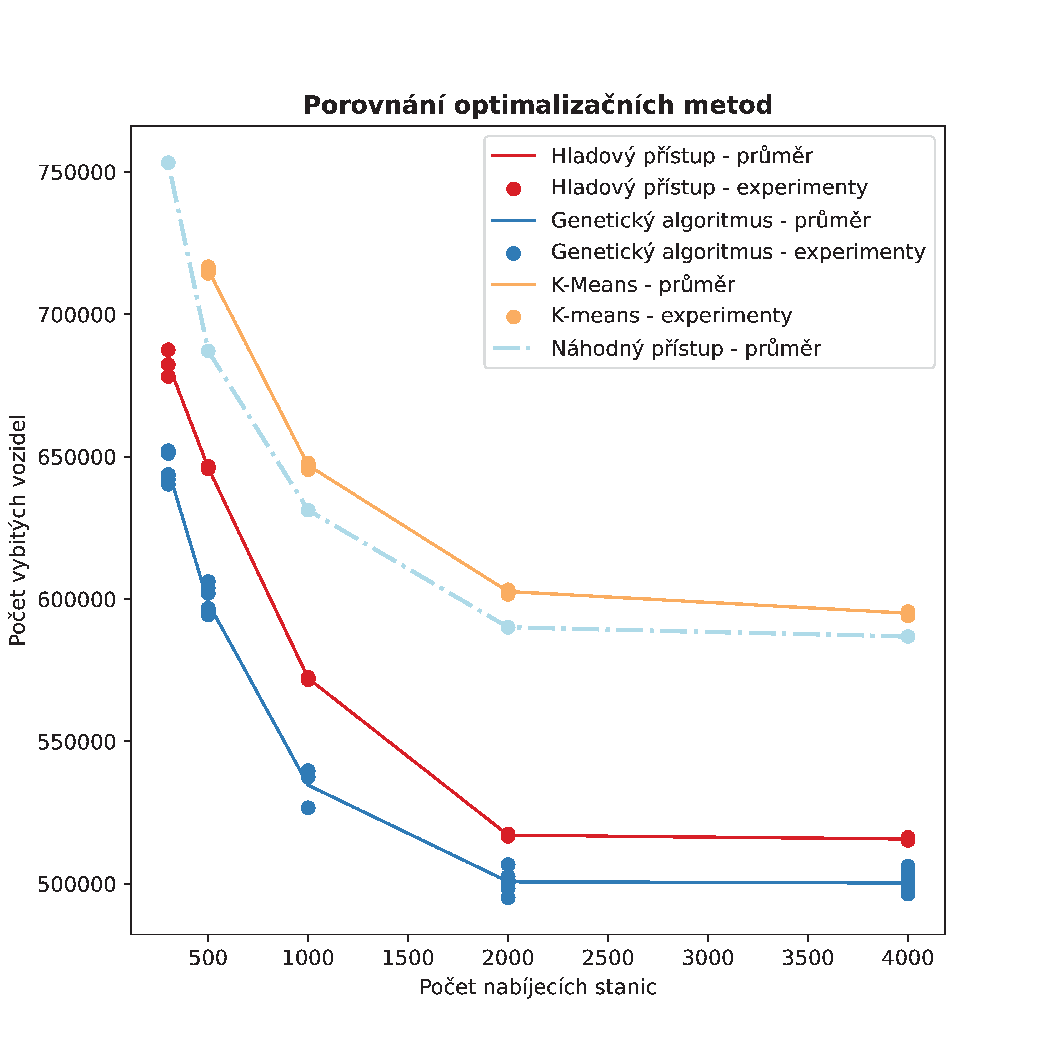
\includegraphics[width=1\linewidth]{img/pdfa-optim_compare.pdf}
    \caption{Porovnání různých optimalizačních metod. Optimalizační metody barevně
    rozlišujeme. Body v grafu znázorňují výsledky jednotlivých experimentů. Čárové
    grafy propojují průměrné hodnoty počtu vybitých vozidel při stejném počtu
    nabíjecích stanic. Čerchovaný čárový graf značí výsledky náhodného přístupu.}
    \label{fig:porovnani_optimalizaci}
\end{figure}



\section{Pomocné nástroje pro analýzu výsledků}

S ohledem na velké množství parametrů simulátoru a výpočetní náročnosti simulace
jsme se rozhodli využít služeb organizace 
Metacentrum\footnote{\url{https://metavo.metacentrum.cz/}}. Za pomoci
této organizace jsme schopni otestovat stovky variant parametrů.
Vzhledem k množštví zkoumaných variant, je ale pro praktické použití potřeba 
zautomatizovat proces nastavování zvolených parametrů a vytváření úloh pro spuštění na 
Metacentru simulací se zvolenými parametry a následnou analýzu výsledků simulací.
K tomuto účelu jsme vytvořili pomocný program v jazyce Python 
(viz. \cref{chap:prilohy}). Tento program připravuje 
potřebné skripty pro spouštění jednotlivých úloh v Metacentru a 
umožňuje jednoduché zobrazení výsledků simulace s možností zkoumání 
námi zvolených parametrů simulace a setřídění výsledků dle zvoleného parametru.

% \chapter{Související práce}
\label{chap:souvisejici_prace}

V této kapitole si popíšeme několik souvisejících prací a stručně popíšeme 
jejich vlastnosti.


Simulátor SUMO\footnote{\url{https://www.eclipse.org/sumo/}} je velmi detailní
simulátor dopravy v rozsahu funkcionalit zdaleka přesahující naši implementaci.
V programu lze do jisté míry simulovat také elektromobily. Pro naše učely je
ale tento program velmi komplexní a práce s optimalizačními algoritmy
by tak byla neprakticky komplikovaná.

Simulátor City Flow\footnote{\url{https://cityflow.readthedocs.io/en/latest/index.html}}
se pyšní především výpočetní efektivitou\footnote{\url{https://cityflow.readthedocs.io/en/latest/introduction.html}}.
Bohužel nenabízí jednoduché uživatelské rozhraní pro rozšíření o metody
potřebné pro naši optimalizaci.

V práci \citet{kmeans_layout} je navržen simulátor dopravy pro následnou 
analýzu navě navrženého optmalizačního algoritmu rozmístění nabíjecích stanic
na území Japonska. Optimalizační algoritmus v práci se snaží minimalizovat 
počet vozidel, kterým se vybila baterie, pomocí posunů nabíjecích stanic směrem
k místům, kde se v minulosti vybila baterie vozidla. Návrh simulátoru naší práce
a optimalizační algoritmus s použití metody K-Means jsou inspirovány zmíněnou
prací.

V práci \citet{niccolai2021optimization} je zkoumáno několik variant evolučních
algoritmů pro optimalizaci rozmístění nabíjecích stanic elektrických vozidel
ve městě Milán. V práci byl porovnáván také hladový přístup rozmísťující 
iterativně nabíjecí stanice na místa lokálních extrémů specificky zadefinované
ztrátové funkce. 

Práce \citet{zhu2016charging} se zabývá optimalizací rozmístění nabíjecích 
stanic v okolí města Peking užitím technik genetického algoritmu. V práci 
jsou porovnávány 2 varianty modelů popisující možné pozice nabíjecích stanic a
je v ní poukázáno, že správná volba modelu ovlivňuje kvalitu řešení optimalizace. 

V práci \citet{kinay2021full} je navžen simulátor pro rozvrhování pozic 
nabíjecích stanic. Problém je zde matematicky popsán. V práci jsou navrženy
2 varianty optimalizací. Jedna minimalizující celkovou cenu rozmístění 
nabíjecích stanic s minimalizací odchylek od původní trasy, druhá optimalizuje
pozice stanic s ohledem na minimalizaci odchylek.
\chapwithtoc{Závěr}
\label{chap:zaver}

V práci jsme navrhli simulátor dopravy speciálně navržen pro snadnou optimalizaci
rozmístění nabíjecí stanic v dopravní síti. A následně zkoumali několik 
vybraných variant optimalizace na mapě dopravní sítě České republiky.

Z důvodu vysoké výpočetní náročnosti zkoumaného problému jsme byli nuceni
některé aspekty simulace značně zjednodušit, což částečně vedlo k 
nerealističnosti výsledků. Ve značné míře jsme například museli zredukovat 
simulovanou silniční síť a simulování cest vozidel na krátké vzdálenosti.
Dalším ze závažných nedostatků simulace je nerealistický počet vozidel,
kterým se vybije baterie během cesty. Hlavním důvodem tohoto nedostatku
je potřeba vhodně zadefinovat chybovou funkci pro optimalizaci problému
(viz. \cref{sec:loss}). Částečně tuto skutečnost způsobuje také velmi
zjednodušený proces volby nabíjecí stanice vozidlem 
(viz. \cref{subsec:zajizdeni_na_nabijecku}).
Tato skutečnost je částečně způsobena nevhodným algoritmem pro volbu nabíjecí
stanice, jenž musel být podstatně zjednodušen v důsledku potřeby výpočetně
efektivního simulátoru. Na základě experimentů, které podrobně popisuje 
kapitola \cref{chap:analysis}, jsme však došli k názoru, že námi navržený 
simulátor popisuje dostatečně kvalitně aspekty dopravní sítě, jenž jsou 
potřebné pro optimalizaci rozmístění nabíjecích stanic. 

Po provedení experimentů jsme došli k závěru, že hladový optimalizační
algoritmus (viz. \cref{sec:greedy}) a především optimalizace pomocí genetického
algoritmu (viz. \cref{sec:genetic_optim}) vykazují lepší výsledky než náhodný
přístup, založený na rozmísťování stanic podle počtu obyvatel v jednotlivých
částech dopravní sítě (např. v genetickém algoritmu se pro 2000 nabíjecích 
stanic snížil počet vozidel s vybitou baterií v simulaci o $\frac{1}{6}$).
Především u optimalizace genetickým algoritmem, pozorujeme, že kvalita řešení 
by se mohla ještě vzrůst při zvýšením počtu generací a velikosti populace.
Tyto výsledky, jsme však vzhledem k výpočetní náročnosti optimalizace nebyli 
schopni ověřit. Na druhou stranu optimalizační algoritmus inspirovaný algoritmem
k-means (\cref{sec:kmeans_optim}) dosahoval dokonce mírně horších výsledků jako
náhodný přístup. Tuto skutečnost si odůvodňujeme velkou mírou aproximace při 
hledání vhodné nabíjecí stanice a malým počtem iterací algoritmu v experimentech.


\section*{Budoucí práce}

Do budoucna se nabízí doimplementovat do simulátoru vhodnější algoritmus pro 
výběr nabíjecí stanice, čímž by se mohla zlepšit realističnost chování vozidel
při jízdě na nabíjecí stanice a výrazně snížit počet vybitých vozidel v 
simulaci.

Dále se nachází potenciál ve zlepšení optimalizační 
algoritmu pomocí algoritmu k-means, který pravděpodobně dosahuje špatných výsledků
z důvodu značné aproximace, s níž algoritmus pracuje. O potenciálu zlepšení jsme
přesvědčeni, protože \citet{kmeans_layout} dosáhli podobným způsobem kvalitních
výsledků.

Dalším potenciálním rozšířením simulátoru je doimplementovat potřebné funkcionality
pro optimalizaci počtu nabíjecích slotů nabíjecích stanic a navržení vhodných
optimalizačních algoritmů řešící tuto problematiku.

Dále je v simulátoru částečně naimplementována funkcionalita pro načítaní a zápis
reprezentace nabíjecích stanic do souboru. Dokončení implementace by nám umožnilo
například optimalizovat již předpřipravené řešení a zkvalitnit tak optimalizaci,
neboť ve všech akuálně používaných optimalizační algoritmech inicializujeme 
optimalizaci na náhodně rozmístěných stanicích.

Také se nabízí potenciál v generování výjezdů a tras cest vozidel založených na 
reálných datech. Čímž bychom mohli zásadně zlepšit realističnost simulovaného
provozu. 

\ifEN
\chapwithtoc{Bibliography}
\else
\chapwithtoc{Seznam použité literatury}
\fi

\printbibliography[heading=none]


\appendix
\chapter{Uživatelská dokumentace}
\label{chap:uzivatelska_dokumentace}

Hlavním cílem programu je na zvolené reprezentaci mapy opakovaně simulovat 
dopravní síť a na základě této simulace optimalizovat rozmístění nabíjecích
stanic s pomocí různých optimalizačních algoritmů. Po ukončení optimalizace
vypíše zvolené relevantní informace o jednotlivých simulacích pro následnou 
analýzu optimalizačních metod. Program také nabízí nastavitelnost široké škály 
parametrů simulátoru dopravy i optimalizačních  metod pro detailnější analýzu.


\section{Příprava před spuštěním}
Rozlišujeme více variant spuštění programu podle OS, který používáme.

Pokud pracujeme v OS \textbf{Windows 10}, pak můžeme použít již předkompilovaný 
program, jenž je součástí přílohy. V tomto případě můžeme program rovnou spustit.
Předkompilovaný spustitelný se nachází v adresáři:

\begin{verbatim}
    Win_executable/
\end{verbatim}

V tomto adresáři se nachází spustitelný program, adresář s předpřipravenou
reprezentací mapy a další pomocné soubory pro správné fungování programu.
Název spustitelného programu je:

\begin{verbatim}
    Traffic_Simulator.exe 
\end{verbatim}

\subsection{Sestavení programu}
Pokud chceme program sestavit, pak je potřeba postupovat v následujících krocích.

\subsubsection{Sestavení pro OS Linux}

Pro sestavení programu v OS Linux potřebujeme
\texttt{CMake 3.11}\footnote{\url{https://cmake.org/}}, 
nebo vyšší (doporučujeme verzi \texttt{3.14+}), překladač podporující \texttt{C++11},
knihovnu \texttt{Boost}\footnote{\url{https://www.boost.org/}} a
Git\footnote{\url{https://git-scm.com/}}.

Nejprve se přesuneme do adresáře s požadovanými zdrojovými kódy.
\begin{verbatim}
    cd source_code/Traffic_Simulator_cmake
\end{verbatim}

Pro konfiguraci spustíme příkaz (přidáme ještě možnost \texttt{-GNinja}, 
pokud používáme Ninja\footnote{\url{https://ninja-build.org/}}).
\begin{verbatim}
    cmake -S . -B build
\end{verbatim}

Pro sestavení programu spustíme příkaz:
\begin{verbatim}
    cmake --build build
\end{verbatim}

Výsledný spustitelný program pak nalezneme:
\begin{verbatim}
    build/apps/Traffic_Simulator
\end{verbatim}

\subsubsection{Sestavení pro OS Windows 10}
Pro sestavení programu v OS Windows 10 potřebujeme překladač podporující 
\texttt{C++11}, Visual Studio 2019\footnote{https://visualstudio.microsoft.com/cs/},
Git a \texttt{vcpkg}\footnote{\url{https://github.com/microsoft/vcpkg}}.

Nejprve se přesuneme do adresáře, kde je uložen nástroj \texttt{vcpkg} a 
nainstalujeme knihovnu Boost.
\begin{verbatim}
    cd $(Absolute_Path_To_vcpkg_Directory)

    .\vcpkg\vcpkg install boost
    .\vcpkg\vcpkg integrate install
\end{verbatim}

Následně se přesuneme do adresáře naší práce a zde do adresáře:

\begin{verbatim}
    cd source_code\Traffic_Simulator_VS
\end{verbatim}
 
Zde nalezenem soubor:
\begin{verbatim}
    Traffic_Simulator.sln
\end{verbatim}

Ten otevřeme v programu Visual Studio 2019, ve kterém projekt sestavíme.

\section{Poznámka k příkladům}
V následujícím textu popisujeme příklady použití programu v OS Linux.
Pokud pracujeme v OS Windows, pak program spouštíme následujícím příkazem
(se zvolenými parametry (viz. \cref{subsec:parametry_programu})):

\begin{verbatim}
    .\Traffic_Simulator.exe
\end{verbatim}

Pokud pracujeme s předpřipravenou mapou z adresáře:
\begin{verbatim}
    preprocesed\_maps
\end{verbatim}

Pak musíme pro fungování příkazů v příkladech, zkopírovat tento adresář do 
adresáře se spustitelným souborem programu. Pokud pracujeme s již
předkompilovaným programem v OS Windows, pak tato operace není nutná.

\section{Formát souborů reprezentujících mapu}
\label{sec:soubor_mapy}

Pro správné fungování programu je potřeba při každém spuštění načíst reprezentaci
mapy (\cref{sec:dopravni_sit}).
Ta je rozdělena do 3 souborů a informace v nich zapsané si nesmějí 
navzájem odporovat. Tyto 3 soubory jsou načítany v pořadí: soubor s reprezentací
křižovatek, soubor s reprezentací silnic a soubor s reprezentací měst.
Vzhledem k obvykle velké objemnosti dat reprezentující dopravní síť je 
doporučeno při přípravě vstupních souborů postupovat podle
kroků, jež popisuje \cref{chap:priprava_mapy}, s pomocí přiložených programů
v adresáři \texttt{map\_preprocessing} práce (viz. \cref{chap:prilohy}).

Pokud chce uživatel pracovat pouze s námi připravenou mapou České republiky, 
jenž podrobněji popisuje \cref{chap:priprava_mapy}, je v adresáři
\texttt{preprocesed\_maps} dodána reprezentace již připravené mapy.
Struktura adresáře je:

\begin{verbatim}
./prepared_graph/
    cities.txt
    combined_nodes.txt
    edges.txt
    prepared_combined_nodes.txt
    prepared_edges.txt
\end{verbatim}

V souborech výše jsou zapsány po řadě, reprezentace měst, reprezentace křižovatek,
reprezentace hran a v souborech s předponou \texttt{prepared\_} je uložena 
předpřipravená reprezentace mapy (bez křižovatek stupně 2) se stejnou reprezentací,
jako v neupravené variantě (reprezentace měst se předpřípravou nemění).

Formát všech vstupních souborů je strukturován po řádcích. V každém souboru
je vždy ignorován první řádek, jehož účelem je popis formátu vstupních dat 
jednotlivých řádků pro každý vstupní soubor. S ohledem na 
přehlednost vstupních dat je doporučeno tento formát vždy dodržovat.
Ve zbytku souboru je postupně na každém řádku reprezentován specifický objekt
mapy, který je určen daným typem souboru. Jakékoli nedodržení formátu
vstupních souborů vede s vysokou pravděpodobností k selhání načítání dat a
není tak umožněna další práce s programem.


\subsection{Soubor reprezentující křižovatky}
\label{subsec:reprezentace_krizovatky}

Předpokládaná hlavička (1. řádek) souboru je:
\begin{Verbatim}
    node_id latitude longitude city_id distance_km 
\end{Verbatim}

Každý řádek, kromě prvního řádku, reprezentuje právě jednu kžižovatku (\cref{def:krizovatka}).
Požadujeme, aby na každém řádku bylo uloženo pět hodnot oddělených mezerou, které 
reprezentují po řadě: identifikační číslo (ozn. ID) křižovatky, zeměpisnou šířku,
v níž se křižovatka nachází, zeměpisnou délku, v níž se křižovatka nachází,
ID města, do něhož křižovatka náleží, a vzdálenost křižovatky od centra tohoto města.

Pro správnou funkci programu je potřeba, aby ID křižovatek byla celá nezáporná 
čísla a aby křižovatky byly v souboru seřazeny vzestupně bez vynechaných hodnot ID.
Tedy pokud např. v souboru existuje vrchol s ID 6, musí být předem definovány
vrcholy s ID v rozmezí od 1 do 5. Dále požadujeme, aby ID křižovatek byly unikátní.
Zeměpisná šířka, zeměpisná délka i vzdálenost města jsou reprezentovány 
desetinným číslem s desetinnou tečkou. ID města je reprezentováno nezáporným
celým číslem, jež musí být zadefinováno v souboru reprezentující města 
(\cref{subsec:reprezentace_mesta}).


Příklad formátu vstupního souboru, jenž reprezentuje křižovatky:
\begin{Verbatim}
    node_id latitude longitude city_id distance_km
    0 50.0354962 14.4080276 1 5.855519633308941 
    1 50.0352373 14.4080465 2 5.883717272182215 
    2 50.0350876 14.4080758 0 5.8998150943334124
    3 50.035876 14.4080352 0 5.8898140943334124
\end{Verbatim}


\subsection{Soubor reprezentující silnice}

Předpokládaná hlavička (1. řádek) souboru je:
\begin{Verbatim}
new_node_id_1 new_node_id_2 length road_type
\end{Verbatim}
Každý řádek, kromě prvního řádku, reprezentuje právě jednu silnici (\cref{def:silnice})
dopravní sítě. Požadujeme, aby na každém řádku byly uloženy čtyři hodnoty oddělené
mezerou reprezentující: ID první křižovatky definující silnici, ID druhé
křižovatky definující silnici, délka silnice a typ silnice.
Předpokládáme, že ID křižovatek jsou v odpovídajícím formátu, 
který je popsán v části pro reprezentaci křižovatek (\cref{subsec:reprezentace_krizovatky})
a zároveň, že křižovatka s ID ze vstupu byla definována a načtena ze souboru 
pro reprezentaci křižovatek.
Délka silnice je reprezentována desetinným číslem s desetinnou tečkou.
\Cref{tab:typy_silnice} vypisuje všechny typy silnice a jejich reprezentaci pro
vstupní soubor.

\begin{table}
\centering\footnotesize\sf
\begin{tabular}{ll}
\toprule
Reprezentace & Popis \\
\midrule
\texttt{m} & dálnice  \\
\texttt{t} & silnice pro motorová vozidla \\
\texttt{p} & silnice 1. třídy nebo  \\
\texttt{o} & jiný druh silnice \\
\bottomrule
\end{tabular}
\caption{Výpis všech variant druhů silnice.}
\label{tab:typy_silnice}
\end{table}
    

Příklad formátu vstupního souboru, jenž reprezentuje silnice:
\begin{Verbatim}
new_node_id_1 new_node_id_2 length road_type
0 1 28.82 t 
1 2 16.777 p
2 3 17.303 m
\end{Verbatim}


\subsection{Soubor reprezentující města}
\label{subsec:reprezentace_mesta}

Předpokládaná hlavička (1. řádek) souboru je:
\begin{Verbatim}
city_id lat lon population
\end{Verbatim}
Každý řádek, kromě 1. řádku, reprezentuje právě 1 město (\cref{def:mesto}).
Požadujeme, aby na každém řádku byly uloženy 4 hodnoty oddělené mezerou reprezentující:
ID města, zeměpisnou šířku, v níž se nachází střed města, zeměpisnou délku, v 
níž se nachází střed města, a počet obyvatel města.
Požadujeme, aby ID města bylo nezáporné celé číslo. Pro zajištění správného 
fungování programu je doporučeno reprezenovat města v souboru v rostoucím
pořadí podle ID města bez opakování a bez vynechaných ID. Tato podmínka 
však není na rozdíl od reprezentace křižovatek nutná.
Zeměpisná šířka a délka jsou reprezentovány desetinným číslem s desetinnou 
tečkou. Populace města je reprezentována nezáporným celým číslem.

Příklad formátu vstupního souboru, jenž reprezentuje  města:
\begin{Verbatim}
city_id lat lon population
0 49.39606475830078 15.590306282043457 51216 
1 49.70147705078125 17.07569122314453 7516 
2 51.02574920654297 15.061005592346191 4259 
\end{Verbatim}


\subsection{Výstupní soubory}

Program také umožňuje zápis aktuálně načtené mapy do souborů ve vstupním formátu
simulátoru. Tato funkcionalita je především užitečná, pokud je předpříprava
původní mapy výpočetně náročná (odstraňování vrcholů stupně 2 nebo 
sjednocování komponent souvislosti). V takovém případě můžeme předpřipravenou
mapu uložit do formátu určeného pro načítání mapy a při opakovaném výpočtu
přeskočit předpřípravu dat a rovnou spustit požadovaný výpočet.


\section{Ovládání programu}

Uživatel interaguje s programem pouze při jeho spuštění, kdy je potřeba
zvolit příslušnou optimalizační metodu, její parametry a parametry simulace.
Před spuštěním programu je potřeba připravit soubory s korektní 
reprezentací mapy (\cref{sec:soubor_mapy}) a specifikovat 
cestu k těmto souborům.


\subsection{Parametry programu}
\label{subsec:parametry_programu}
Při spuštění programu zadáváme do terminálu parametry, kterými specifikujeme
požadované chování simulátoru. Tyto parametry zapisujeme ve formě přepínačů za
příkaz spouštějící program. Tyto přepínače popisujeme v tabulkách rozdělených
podle jejich funkce.
\Cref{tab:prepinace_pomocne} popisuje pomocné přepínače programu, 
\cref{tab:prepinace_soubory} popisuje přepínače pro specifikování vstupních a 
výstupních souborů, \cref{tab:prepinace_simulace} popisuje přepínače pro volbu
parametrů simulace, \cref{tab:prepinace_optimalizace} popisuje přepínače pro 
volbu obecných vlastností typických pro všechny optimalizační metody,
\cref{tab:prepinace_greedy} popisuje přepínače pro volbu parametrů hladové optimalizace,
\cref{tab:prepinace_genetic}, popisuje přepínače pro volbu parametrů optimalizace genetickým
algoritmem, \cref{tab:prepinace_kmeans} popisuje přepínače pro volbu parametrů optimalizace
pomocí algoritmu k-means a \cref{tab:prepinace_volba_optim} popisuje přepínače pro volbu
optimalizační metody.

\begin{table}
\centering\footnotesize\sf
\begin{tabular}{p{0.15\linewidth} p{0.75\linewidth}}
\toprule
Příkaz & Popis funkce \\
\midrule
\texttt{help} & Vypíše všechny možnosti parametrů programu. \\
\texttt{logs} & Program bude vypisovat podrobné informace o průběhu simulace 
(pro ladění progamu). \\
\bottomrule
\end{tabular}
\caption{Popis pomocných přepínačů v programu.}
\label{tab:prepinace_pomocne}
\end{table}


\begin{table}
\centering\footnotesize\sf
\begin{tabular}{p{0.30\linewidth} p{0.6\linewidth}}
\toprule
Příkaz & Popis funkce \\
\midrule
\texttt{nodeCityFile arg} & Cesta k vstupnímu souboru s reprezentací křižovatek. 
V případě nespecifikované hodnoty je zvolena cesta:
\texttt{prepared\_graph/combined\_nodes.txt} \\
\texttt{edgesFile arg} & Cesta k vstupnímu souboru s reprezentací silnic.
V případě nespecifikované hodnoty je zvolena cesta:
\texttt{prepared\_graph/edges.txt} \\
\texttt{citiesFile arg} & Cesta k vstupnímu souboru s reprezentací měst. 
V případě nespecifikované hodnoty je zvolena cesta:
\texttt{prepared\_graph/cities.txt} \\
\texttt{addedEdgesFile arg} & Cesta k výstupnímu souboru pro uložení reprezentace 
přidaných hran pro vytvoření souvislého grafu. 
V případě nespecikované hodnoty je zvolena cesta:
\texttt{prepared\_graph/added\_edges.txt} \\
\texttt{preparedNodesFile arg} & Cesta k výstupnímu souboru pro uložení reprezentace
vrcholů upraveného grafu po eliminaci vrcholů stupně 2.
V případě nespecikované hodnoty je zvolena cesta:
\texttt{prepared\_graph/prepared\_combined\_nodes.txt} \\
\texttt{preparedEdgesFile arg} & Cesta k výstměupnímu souboru pro uložení reprezentace
hran upraveného grafu po eliminaci vrcholů stupně 2 
V případě nespecikované hodnoty je zvolena cesta:
\texttt{prepared\_graph/prepared\_edges.txt}\\
\texttt{savePrepared} & Parametr specifikující, zda uložit předpřipravenou 
reprezentaci mapy. \\
\bottomrule
\end{tabular}
\caption{Popis přepínačů pro specifikování vstupních a výstupních souborů.}
\label{tab:prepinace_soubory}
\end{table}


\begin{table}
\centering\footnotesize\sf
\begin{tabular}{p{0.43\linewidth} p{0.5\linewidth}}
\toprule
Příkaz & Popis funkce \\
\midrule
\texttt{simulationTime arg} & Doba simulace v minutách. \\
\texttt{segmentLength arg} & Délka hrany grafu v kilometrech. \\
\texttt{numClosestStations arg} & Počet nabíjecích stanic, které jsou zvažovány 
    při plánování cesty vozidla na nabíjecí stanici. \\
\texttt{carConsumption} & Spotřeba baterie vozidla v procentech kapacity za minutu. \\
\texttt{numStations arg} & Celkový počet nabíjecích stanic v simulaci. \\
\texttt{stationCapacity arg} & Počet nabíjecích slotů na každé stanici. \\
\texttt{exponentialLambdaCities arg} & Parametr pro generování cílového města vozidla.
    Hodnota je rovna $\frac{1}{d}$, kde $d$ je střední hodnota vzdálenosti 
    cílového města od startu v kilometrech. \\
\texttt{exponentialLambdaDepartures arg} & Parametr pro generování času výjezdu
    následujícího vozidla. Hodnota je rovna $\frac{1}{t}$, kde $t$ je střední 
    hodnota času následujícího výjezdu vozidla v minutách. \\
\texttt{endCityRatio arg} & Parametr specifikující důležitost vzdálenosti cílového
    města vůči počtu obyvatel při generování cílového města 
    (viz. \cref{def:pravdepodobnost_ciloveho_mesta}). Pokud $<1$, pak je
    počet obyvatel důležitější. Pokud $=1$, pak jsou oba parametry stejně důležité.
    Pokud $>1$, pak je důležitější vzdálenost města. \\
\texttt{batteryTresholdLambda arg} & Hodnota $\frac{1}{b}$, kde $b$ je střední 
    hodnota hladiny baterie specifikující, o kolik průměrně převyšuje hladina baterie v době
    rozhodnování nejnižší možnou hranici pro rozhodnutí, zda jet nabíjet, v moment rozhodnutí
    (viz. \cref{subsec:zajizdeni_na_nabijecku}). \\
\texttt{carBatteryMean arg} & Střední hodnota počáteční hladiny baterie. \\
\texttt{carBatteryDeviation arg} & Směrodatná odchylka počáteční hladiny baterie vozidla. \\
\texttt{carStartBatteryBottomLimit arg} & Minimální hladina baterie vozidla při výjezdu. \\
\texttt{chargingTreshold arg} & Nejnižší možná hladina baterie pro rozhodnutí,
    zda vyrazit na nabíjecí stanici (viz. \cref{subsec:zajizdeni_na_nabijecku}). \\
\texttt{notChargingTreshold arg} & Nejvyšší hladina pro rozhodnutí, zda vyrazit na 
    nabíjecí stanici (viz. \cref{subsec:zajizdeni_na_nabijecku}). \\
\texttt{batteryTolerance arg} & Nejnižší možná očekávaná hladina baterie v cíli, 
    kdy se při rozhodování, rozhodnout nezajet na nabíjecí stanici 
    (viz. \cref{subsec:zajizdeni_na_nabijecku}). \\
\texttt{carVelocity arg} & Průměrná rychlost všech vozidel v kilometrech za minutu. \\
\texttt{chargingWaitingTime arg} & Doba čekání na úplné nabití baterie v minutách.  \\
\texttt{meanChargingLevel arg} & Očekávaná střední hodnota hladiny baterie, jež
    je nabíjena na nabíjecích stanicích (pro odhad doby čekání nabíjení ve frontě).  \\
\bottomrule
\end{tabular}
\caption{Popis přepínačů pro specifikování parametrů simulátoru.}
\label{tab:prepinace_simulace}
\end{table}


\begin{table}
\centering\footnotesize\sf
\begin{tabular}{p{0.42\linewidth} p{0.51\linewidth}}
\toprule
Příkaz & Popis funkce \\
\midrule
\texttt{lossDifferenceTreshold arg} & Minimální rozdíl ztrátové funkce pro 
pokračování v optimalizaci (pro vybrané optimalizační metody). \\
\texttt{stationNumberParameter arg} & Parametr počtu stanic při výpočtu ztrátové 
funkce (viz. \cref{sec:loss}).\\
\texttt{runDownParameter arg} & Parametr počtu vozidel, kterým se vybila baterie,
pro výpočet ztrátové funkce (viz. \cref{sec:loss}).\\
\texttt{durationParameter arg} & Parametr průměrné doby cestování v minutách pro
výpočet ztrátové funkce (viz. \cref{sec:loss}).\\
\texttt{batteryDifferenceParameter arg} & Parametr průměrného rozdílu hladin 
baterie pro výpočet ztrátové funkce (viz. \cref{sec:loss}).\\
\texttt{waitingTimesParameter arg} & Parametr průměrné čekací doby na nabíjecích
stanicích pro výpočet ztrátové funkce (viz. \cref{sec:loss}).\\
\bottomrule
\end{tabular}
\caption{Popis přepínačů pro specifikování obecných vlastností optimalizace.}
\label{tab:prepinace_optimalizace}
\end{table}


\begin{table}
\centering\footnotesize\sf
\begin{tabular}{p{0.35\linewidth} p{0.58\linewidth}}
\toprule
Příkaz & Popis funkce \\
\midrule
\texttt{greedyMaxIterations arg} & Maximální počet iterací algoritmu. \\
\texttt{greedyNumThrowAway arg} & Maximální rozdíl počtu stanic mezi iteracemi algoritmu. \\
\bottomrule
\end{tabular}
\caption{Popis přepínačů pro specifikování parametrů hladové optimalizace (viz. \cref{sec:greedy}).}
\label{tab:prepinace_greedy}
\end{table}


\begin{table}
\centering\footnotesize\sf
\begin{tabular}{p{0.52\linewidth} p{0.41\linewidth}}
\toprule
Příkaz & Popis funkce \\
\midrule
\texttt{geneticPopulatioSize arg} & Velikost populace. \\
\texttt{geneticNumGenerations arg} & Počet generací. \\
\texttt{geneticNumBestSelection arg} & Počet nejlepších jedinců pro zkopírování
    do následující generace. \\
\texttt{geneticTournamentSelectionTreshold arg} & Pravděpodobnost výběru lepšího
    jedince v turnajové selekci. \\
\texttt{geneticMutationTreshold arg} & Pravděpodobnost mutace nabíjecí stanice. \\
\texttt{geneticMemberSizeVariance arg} & Směrodatná odchylka rozdílu velikosti 
    nového jedince a jeho rodiče pro mutaci velikosti jedince. \\
\bottomrule
\end{tabular}
\caption{Popis přepínačů pro specifikování parametrů optimalizace genetickým algorimem
    (viz. \cref{sec:genetic_optim}).}
\label{tab:prepinace_genetic}
\end{table}


\begin{table}
\centering\footnotesize\sf
\begin{tabular}{p{0.46\linewidth} p{0.47\linewidth}}
\toprule
Příkaz & Popis funkce \\
\midrule
\texttt{kMeansNumIterationsOneRun arg} & Počet iterací jednoho běhu algorimu k-means. \\
\texttt{kMeansNumGenerations arg} & Počet generací modelů. \\
\bottomrule
\end{tabular}
\caption{Popis přepínačů pro specifikování parametrů optimalizace algoritmem k-means 
    (viz. \cref{sec:kmeans_optim}).}
\label{tab:prepinace_kmeans}
\end{table}


\begin{table}
\centering\footnotesize\sf
\begin{tabular}{p{0.17\linewidth} p{0.76\linewidth}}
\toprule
Příkaz & Popis funkce \\
\midrule
\texttt{randomModels} & Spustí pevný počet simulací na modelech s náhodně 
rozmístěnými nabíjecími stanicemi. \\
\texttt{greedy} & Spustí optimalizaci hladovým algoritmem. \\
\texttt{genetic} & Spustí optimalizaci genetickým algorimem. \\
\texttt{kMeans} & Spustí optimalizaci algoritmem K-Means. \\
\bottomrule
\end{tabular}
\caption{Popis přepínačů pro volbu optimalizační metody.}
\label{tab:prepinace_volba_optim}
\end{table}


\subsection{Příklad spouštění programu}
V této sekci uvádíme příklad spuštění programu se vstupními soubory. Po řadě pro
křižovatky, silnice a města s názvy:
\begin{Verbatim}
    prepared_graph/combined_nodes.txt
    prepared_graph/edges.txt
    prepared_graph/cities.txt
\end{Verbatim}

Dále uvádíme výstupní soubory. Po řadě pro soubor s nově přidanými hranami
po sloučení komponent souvislosti, pro reprezentaci vrcholů z předpřipraveného grafu 
a pro reprezentaci hran z předpřipraveného grafu:
\begin{Verbatim}
    prepared_graph/added_edges.txt, 
    prepared_graph/prepared_nodes_new.txt
    prepared_graph/prepared_edges_new.txt
\end{Verbatim}

Dále v tomto příkladě volíme čas simulace 100 minut, celkový počet stanic 300 a
počet generací genetického algoritmu 3. Nakonec specifikujeme, že chceme spustit 
optimalizaci genetickým algoritmem a uložit předpřipravenou mapu. Další parametry
jsou zvoleny automaticky, podle výchozí hodnoty nastavené v programu, kterou lze
dohledat příkazem:

\begin{Verbatim}
    ./Traffic_Simulator --help
\end{Verbatim}

Optimalizaci na parametrech popsaných výše spustíme příkazem:

\begin{Verbatim}
./Traffic_Simulator \
--nodeCityFile="prepared_graph/combined_nodes.txt" \
--edgesFile="prepared_graph/edges.txt" \
--citiesFile="prepared_graph/cities.txt" \
--addedEdgesFile="prepared_graph/added_edges.txt" \
--preparedNodesFile="prepared_graph/prepared_combined_nodes_new.txt" \
--preparedEdgesFile="prepared_graph/prepared_edges_new.txt" \
--simulationTime=100 \
--numStations=300 \
--geneticNumGenerations=3 \
--genetic \
--savePrepared
\end{Verbatim}


Pokud zvolíme vstupní soubory (křižovatek, silnic a města):

\begin{Verbatim}
    prepared_graph/prepared_combined_nodes.txt
    prepared_graph/prepared_edges.txt
    prepared_graph/cities.txt
\end{Verbatim}

Pokud nechceme ukládat předpřipravenou podobu grafu a parametry volíme stejně jako v minulém
případě, pak příkaz pro spuštění vypadá následovně:

\begin{Verbatim}
    ./Traffic_Simulator \
    --nodeCityFile="prepared_graph/prepared_combined_nodes.txt" \
    --edgesFile="prepared_graph/prepared_edges.txt" \
    --citiesFile="prepared_graph/cities.txt" \
    --simulationTime=100 \
    --numStations=300 \
    --geneticNumGenerations=3 \
    --genetic 
\end{Verbatim}


\section{Výstup programu}
První část výstupu programu je vždy výpis použitých parametrů. Část tohoto
výpisu může vypadat například následovně:

\begin{Verbatim}
Save prepared is: 0
Edges: prepared_graph/prepared_edges.txt
Node City: prepared_graph/prepared_combined_nodes.txt
Cities: prepared_graph/cities.txt
Simulation time: 1000
Length of the edge segment: 1
Number of closest stations: 10
Car consumtion: 0.001
Number of charging stations: 500
Capacity of the charging station: 1
...
\end{Verbatim}

Následuje část kontrolních zpráv o procesu eliminace křižovatek stupně 2. 
Program vždy po eliminaci 10000 křižovatek stupně 2 vypíše
informaci o úspěšném průběhu procesu eliminace křižovatek. 
Příklad tohoto výpisu může vypadat následovně:

\begin{Verbatim}
Iteration: 0 Vertices of degree 2 merged and deleted.
Iteration: 10000 Vertices of degree 2 merged and deleted.
Iteration: 20000 Vertices of degree 2 merged and deleted.
Iteration: 30000 Vertices of degree 2 merged and deleted.
Iteration: 40000 Vertices of degree 2 merged and deleted.
Iteration: 50000 Vertices of degree 2 merged and deleted.
Iteration: 60000 Vertices of degree 2 merged and deleted.
Iteration: 70000 Vertices of degree 2 merged and deleted.
Iteration: 80000 Vertices of degree 2 merged and deleted.
Iteration: 90000 Vertices of degree 2 merged and deleted.
Iteration DONE
\end{Verbatim}


Dále následuje posloupnost kontrolních zpráv o slučování komponent 
souvislosti, která je zakončena informací o spuštění zvolené optimalizační metody. 
Tato posloupnost může vypadat následovně (pro spuštění hladové optimalizační
metody):

\begin{Verbatim}
Total number of components: 16
Total number of components: 15
Total number of components: 14
Total number of components: 13
Total number of components: 12
Total number of components: 11
Total number of components: 10
Total number of components: 9
Total number of components: 8
Total number of components: 7
Total number of components: 6
Total number of components: 5
Total number of components: 4
Total number of components: 3
Total number of components: 2
Total number of components: 1
Running greedy algorithm.
\end{Verbatim}

Dále následuje výpis kontrolních zpráv o běhu simulace po každých 
10 odsimulovaných minutách, který je zakončen výsledky simulace a informací
o hodnotě ztrátové funkce. Tento výpis se periodicky opakuje pro každou
spuštěnou simulaci. 
Níže uvádíme příklad výpisu jednoho běhu simulace pro dobu 100 minut.

\begin{Verbatim}
Time 10 elapsed!
Time 20 elapsed!
Time 30 elapsed!
Time 40 elapsed!
Time 50 elapsed!
Time 60 elapsed!
Time 70 elapsed!
Time 80 elapsed!
Time 90 elapsed!
Time 100 elapsed!
Number of stations: 500
Number of run down batteries: 654393
Average traveling duration: 98.0642
Average battery difference between start and end: -0.345312
Average waiting times in charging station: 165.868
------------------------------------------------------
Model loss: 6.54896e+07
\end{Verbatim}

Po skončení všech simulací je program zakončen finálním výpisem informací o
modelu s nejmenší hodnotou ztrátové funkce, nebo v případě volby 
\texttt{randomModels} výpisem aritmetického průměru hodnot popisující vlastnosti simulace.

Speciálním případem je optimalizace za pomoci genetického algoritmu, kde jsou
před finálním výpisem vypsány hodnoty ztrátové funkce všech modelů použitých v průběhu
optimalizace. Část finálního výpisu genetického algoritmu před výpisem informací o nejlepším
modelu může pro 3 generace a velikost populace 3 vypadat následovně:

\begin{Verbatim}
Algorithm finished
Losses for the generation: 0
Loss: 7.58681e+07
Loss: 7.5309e+07
Loss: 7.55552e+07
Losses for the generation: 1
Loss: 7.44727e+07
Loss: 7.56497e+07
Loss: 7.46101e+07
Losses for the generation: 2
Loss: 7.55472e+07
Loss: 7.50069e+07
Loss: 7.56775e+07

Total best loss is: 7.44727e+07
\end{Verbatim}

Finální výpis nejlepších výsledků všech optimalizačních metod může vypadat následovně:

\begin{Verbatim}
Best model info:
------------------------------------------------------
Number of stations: 101
Number of run down batteries: 733511
Average traveling duration: 100.09
Average battery difference between start and end: -0.34632
Average waiting times in charging station: 203.302
------------------------------------------------------
Model loss: 7.33615e+07
\end{Verbatim}

Tento výpis nám říká, že v nejlepším modelu bylo použito $101$ nabíjecích stanic,
počet vozidel, kterým došla baterie je $733511$, průměrná doba cestování vozidla
v minutách je $100.09$, průměrný rozdíl počáteční a koncové hladiny baterie je 
$-0.34632$ (záporná hodnota znamená, že vozidlo dojelo do cíle s vyšší hladinou
baterie, než s jakou vyjíždělo), průměrný čas čekání vozidel na nabíjecích stanicí
než se dostanou na řadu je $203.302$ a nakonec hodnota ztrátové funkce modelu
je $7.33615e+07$.
\chapter{Programátorská dokumentace}
\label{chap:prog_dok}

Účelem této části je především vysvětlit vzájemnou propojenost jednotlivých
tříd programu a vysvětlit jeho fungování v rámci celku. Podrobné informace o
konkrétních metodách jednotlivých tříd jsou popsány v podrobné dokumentaci
programu (viz. \cref{chap:prilohy}).


\section{Struktura programu}
Program je strukturován do vrstev tak, aby byla zajištěna jednoduchá práci s programem
na různých úrovni abstrakce. 

Uživatel pracuje pouze s nejabstraktnější vrstvou,
kterou je třída \texttt{Optimizer}, jež spravuje veškerou logiku spojenou s optimalizací.
Tato třída obaluje třídu \texttt{TimeTable}, jež je zodpovědná za správné fungování
diskrétní simulace a vytváři abstrakci pro třídu \texttt{TrafficSimulator}. Třída
\texttt{TrafficSimulator} je zodpovědná především za generování
událostí simulace (např. následující výjezd vozidla, odkud vozidlo vyjede a 
kam směřuje apod.) a propojení všech objektů simulace. Důležitým aspektem této 
vrsty je správa načítání mapy. Třída spravuje objekty třídy \texttt{MapReader}
a \texttt{GraphAdjuster} zodpovědné za správné předzpracování mapy. Dále je zodpovědná
za veškeré objekty abstraktní třídy \texttt{Vehicle}, které reprezentují vozidla v 
simulaci. V neposlední řadě také vytváří abstrakci pro třídy \texttt{Map}, která 
reprezentuje nejnižší vrstvu programu. Třída
\texttt{Map} je zodpovědná za veškeré grafové operace a veškeré operace pracující s 
reálnou zeměpisnou pozicí. Její součástí je objekt knihovny \texttt{boost}
s názvem \texttt{graph\_} reprezentující graf silniční sítě. Dále třída shlukuje 
informace o nabíjecích stanicích (reprezentované pomocí třídy \texttt{ChargingStation})
a městech náležících do simulované oblasti. 

Součástí programu je také řada dalších tříd pokrývající pomocné operace programu.
Některé z nich jsme již zmínili (\texttt{MapReader}, \texttt{GraphAdjuster}, 
\texttt{Vehicle}, 
\texttt{ChargingStation}). Za zmínku stojí ještě třídy \texttt{Car}, jež je potomkem třídy
\texttt{Vehicle} reprezentující typ vozidla "auto" (viz. \cref{subsec:druhy_vozidel}),
\texttt{Edge}, která pokrývá funkcionalitu a vlastnosti silnice v mapě (viz. \cref{def:silnice})
a \texttt{Node}, jež plní funkci křižovatek na mapě (viz. \cref{def:krizovatka}).
Zbylé třídy slouží především pro shlukování souvisejících informací 
(parametry simulátoru, optimalizací, vlastnosti nabíjecích stanic, modelu apod.).

Jedinou vyjímkou, jež není součástí struktury výše je část pracující s 
parametry programu, jež je realizována pomocí knihovny \texttt{boost}. Přesněji pomocí
funkcionalit z \texttt{program\_options}.


\section{Třída Optimizer}

Třída \texttt{Optimizer} je hlavní třídou celého programu, která na základě 
uživatelských vstupů spouští a realizuje zvolenou optimalizaci. Vytváří 
abstrakci nad třídou \texttt{TimeTable}, jež používáme pro spouštění simulací. 
Do rozhraní třídy náleží metody spouštějící optimalizační algoritmy:

\begin{verbatim}
    GreedyAlgorithm
    GeneticAlgorithm
    KMeansAlgorithm
\end{verbatim}

Metoda, jež počítá ztrátovou funkci modelu po uběhnutí simulace:
\begin{verbatim}
    ModelLoss
\end{verbatim}

A metoda, která opakovaně simuluje provoz na náhodně vygenerovaném modelu:
\begin{verbatim}
    RunMultipleSimulations
\end{verbatim}

Tato metoda slouží pro analýzu optimalizačních metod pro porovnání metod s 
náhodným přístupem. \Cref{chap:optim} nabízí podrobnější popis jednotlivých 
optimalizačních metod a ztrátové funkce. Dále třída obsahuje řadu privátních 
metod zajišťujících správnou funkčnost hlavních metod popsaných výše. Více informacím
je specifikováno v podrobné dokumentaci (viz. \cref{chap:prilohy}).

\section{Třída TimeTable}

Třída \texttt{TimeTable} je třída zodpovědná za správné fungování diskrétní
simulace. Vytváří abstrakci třídy \texttt{TrafficSimulator} a slouží jako rozhraní pro
zisk informací o vlastnostech simulace (pro analýzu optimalizačních metod). 
Do jejího rozhraní náleží především funkce spravující diskrétní simulaci.
Další skupinou metod této třídy jsou metody s předponou \texttt{Get}, 
s jejíž pomocí jsme schopni získat relevantní informace o simulaci.
Jediná metoda, jež nenáleží do zmíněných skupin je \texttt{LoadMap}. Ta slouží
jako zprostředkovatel žádosti o načtení mapy a spouští příslušné
metody ve třídě \texttt{TrafficSimulator}.

\Cref{chap:prubeh_simulace} nabízí podrobnější popis fungování diskrétní
simulace.


\section{Třída TrafficSimulator}

Třídu \texttt{TrafficSimulator} lze považovat za jádro celého simulátoru, jejíž funkce
je spravovat objekty simulace. V rámci simulace je zodpovědná především za
generování náhodných jevů (pozice nabíjecích stanic, generování vozidel, doby 
následující akce apod.) (viz. \cref{subsec:generovani_vozidel}), 
jež je zastoupeno metodami s předponou \texttt{Generate}. Pomocí této třídy jsou v simulaci
spravovány objekty vozidel (potomci třídy \texttt{Vehicle}). Zásadní vlastností této třídy
je vytváření rozhraní pro práci s třídou \texttt{Map}, jež pokrývá veškeré grafové 
operace programu. S třídou \texttt{Map} také úzce souvisí třídy 
\texttt{MapReader} a \texttt{GraphAdjuster}, sloužící pro načtení a předpřípravu
uživatelské reprezentace mapy do formátu, jenž je uložen
ve třídě \texttt{Map}. \Cref{sec:soubor_mapy} podrobně popisuje formát vstupních souborů.


\section{Třída Map}

Třída \texttt{Map} je technicky nejkomplexnější část programu. Slouží
jako rozhraní pro veškeré grafové operace a operace, jež pracují s reálnou
geografickou pozicí na mapě. Graf dopravní sítě je reprezentován pomocí 
příslušných objektů grafové části knihovny \texttt{boost}. Dále jednotlivé křižovatky 
(\cref{def:krizovatka}) a silnice (\cref{def:silnice}) jsou navíc reprezentovány 
vlastními objekty třídy \texttt{Node} (křižovatky) a \texttt{Edge} (silnice). 
Třída také sdružuje všechny nabíjecí stanice (\cref{def:nabijeci_stanice}) vyskytující 
se v mapě (reprezentovány třídou \texttt{ChargingStation}) a informace o rozmístění a 
populaci měst (\cref{def:mesto}) v simulované oblasti.

Třída obsahuje metody pro spravování podoby grafu, informací o nabíjecích 
stanicích a městech. Tyto funkcionality pokrývají metody s předponou \texttt{Add} a 
\texttt{Set}. Dále jsou zde metody pro získávání informací o objektech mapy začínající
příponou \texttt{Get} a \texttt{Exist} a metody přímo související s diskrétní simulací a 
optimalizací (\texttt{ResetSimulation} a \texttt{SimulateVehiclePassedThroughEdge}). Poslední
skupinou metod jsou nejkomplexnější operace třídy pracující s grafem, či mapou.


\subsection{Operace na mapě}

S ohledem na řešený problém je velmi důležitým aspektem návrhu hledání 
nejkratších cest. Program umí pracovat s 2 variantami algoritmu pro hledání
nejkratších cest v grafu. Těmi jsou Dijkstrův algoritmus, jenž je využívám
především pro hledání vzdáleností v grafu (např. v K-Means), a A-Star 
(\cref{sec:a_star}), jenž je používám v diskrétní simulaci pro hledání 
nejvýhodnější cesty vozidla (viz. \cref{subsec:hledani_trasy}).
Jako heuristika algoritmu A-Star je zvolena reálná geografická vzdálenost
mezi křižovatkami, která je spočítána pomocí příslušných vztahů pro výpočet
sférické vzdálenosti (viz. \cref{sect:zem_souradnice}). 

Dijkstrův algoritmus, algoritmus A-Star a výpočet sférické vzdálenosti je realizován
pomocí metod (ve stejném pořadí, jak jsou vypsány):

\begin{Verbatim}
    DijkstraFindDistances
    FindShortestPath
    ComputeSphericalDistance
\end{Verbatim}

Speciální metodou související s výpočtem nejkratší cesty v grafu je:

\begin{Verbatim}
    FindVehiclePath
\end{Verbatim}

Ta hledá nejkratší cestu mezi vrcholy, ale bere také v úvahu potřebu návštěvy nabíjecí
stanice, z níž vybere heuristicky tu nejvhodnější (viz. \cref{subsec:zajizdeni_na_nabijecku}).

Další metodou pracující s grafy je metoda pro hledání komponent souvislosti, 
využívaná v předpřípravě mapy pro simulaci.

\begin{Verbatim}
    TestComponents
\end{Verbatim}

Třída také obsahuje metodu hledající nejbližšího města od křižovatek a nejbližší
nabíjecí stanice od středů měst:

\begin{Verbatim}
    FindCityNodes
    FindCitiesNearestChargingStations
\end{Verbatim}


\section{Třídy objektů mapy}

Mezi třídy reprezentující objekty na mapě patří reprezentace křižovatek (\texttt{Node}),
silnic (\texttt{Edge}) a nabíjecích stanic (\texttt{ChargingStation}). 
Tyto třídy slouží především pro udržování informací o vlastnostech objektů,
obsahují však také jednoduchou logickou vrstvu pokrývající především správnou 
inicializaci, či aktualizaci informací v průběhu simulace. Třída \texttt{ChargingStation}
také pokrývá logickou vrstvu související s nabíjením vozidel (spravuje čekání 
vozidel v řadě, doby nabíjení apod.).


\section{Třídy pro načítání a předpřípravu dat}

Reprezentaci mapy je potřeba na začátku programu načíst z předpřipraveného 
formátu (viz. \cref{sec:soubor_mapy}) a řádně zpracovat do podoby s níž bude
simulátor dále pracovat (\cref{def:graf_site}). K tomuto
účelu slouží třídy \texttt{MapReader} a \texttt{GraphAdjuster}.

\subsection{Třída MapReader}
Třída \texttt{MapReader} převádí vstupní reprezentaci dat do požadovaného formátu
pomocí metod s předponou \texttt{Load}. Nejdůležitější metodou tohoto typu je metoda
\texttt{LoadMap}, jež načte veškeré potřebné informace a provede také předpřípravu 
mapy pro správné fungování simulátoru a zlepšení efektivity. Zmíněné úpravy
provádí s pomocí třídy \texttt{GraphAdjuster}. Dalším charakteristickou vlastností třídy
\texttt{MapReader} je možnost uložení aktuální reprezentace mapy (po předpřípravě mapy)
do souboru v požadovaném vstupním formátu pro efektivnější opakované 
načítání mapy. Mezi tyto metody patří takové, jejichž přípona je \texttt{Write}.

Třída nabízí možnost načítat a zapisovat také reprezentaci všech nabíjecích
stanic modelu metodami:

\begin{verbatim}
    LoadChargingStations
    WriteStations
\end{verbatim}

\subsection{Třída GraphAdjuster}
Vzhledem k typicky velkému rozměru vstupních dat je pravděpodobné, že výsledná
reprezentace mapy nebude splňovat veškeré potřebné vlastnosti nutné k správnému
chování programu, či bude jejich reprezentace zbytečně neefektivní. 
Typickými příklady tohoto problému je rozpad grafu na více komponent souvislosti
či vznik vrcholů stupně 2. Podrobněji tuto problematiku popisuje \cref{chap:priprava_mapy}. 

Řešení těchto potíží zajisťuje třída \texttt{GraphAdjuster} úzce pracující s
třídou \texttt{MapReader}. Ta po načtení grafu zkontroluje zda je graf souvislý
a pokud není, pak jej převede do souvislé podoby 
(viz. \cref{subsubsec:souvislost_grafu}). Dále se také zbavuje veškerých vrcholů 
stupně 2, čímž výrazně zefektivňuje budoucí simulaci (viz. \cref{subsec:problemy_modelu}). 
Operace jsou realizovány metodami:

\begin{verbatim}
    MergeTwoComponents
    MergeDegreeTwoVertices
\end{verbatim}


\section{Třída Vehicle}

Třída \texttt{Vehicle} je třída zahrnující veškeré informace o daném vozidle (\cref{sec:vozidla}),
s jejíž pomocí je možné simulovat chování vozidel a příslušně tak upravovat simulátor.
Při návrhu této třídy byla snaha co nejobecněji vyjádřit chování vozidel 
různých druhů a jednotlivé druhy vozidel simulace následně reprezentovat třídou,
jež je potomkem \texttt{Vehicle}. V naší implementaci je zvolen pouze jeden typ vozidla a 
to typ \texttt{Car}, jehož specifickou vlastností je, že po dosažení cílové 
destinace vrací zpět do místa výjezdu (viz. \cref{subsec:druhy_vozidel}).

Metody třídy \texttt{Vehicle} slouží převážně k získávání informací o vozidle
jinými objekty (např. aktuální stav baterie, aktuální pozice, 
zda míří na nabíjecí stanici apod.), případně k nastavování stavových parametrů 
vozidel (míří na nabíjecí stanici, začalo čekat v řadě na nabíjení apod.)
Objekty třídy jsou také schopny spočítat čas a hladinu baterie po průjezdu
silnicí, dokonce i posloupnosti silnic (celé cesty). Tyto informace jsou důležité
především pro diskrétní simulaci (\cref{chap:prubeh_simulace}) a při rozhodování, 
zda je potřeba jet na nabíjecí stanici (\cref{subsec:zajizdeni_na_nabijecku}).
Zbylé metody slouží pro simulaci akcí vozidel. Je zde metoda pro aktualizaci
trasy vozidla a nabití vozidla:

\begin{verbatim}
    UpdateVehiclePath
    ChargeBattery
\end{verbatim}

Nakonec obsahuje třída i metody, jež řádně simulují průjezd vozidla po silnici. 
V tomto případě jsou naimplementovány 3 varianty, jež řeší všechny možné varianty
průjezdu vozidla (\cref{subsec:udalost_presunu}) po silnici 
(průjezd silnice, výjez z vniřku ven, cesta uvnitř silnice).


\section{Pomocné třídy}

Zbylé třídy implementace slouží především k zapouzdření souvisejících informací,
jako jsou například parametry simulátoru, optimalizací, informace o pozicích na mapě, 
shrnující popis modelu a mnoho dalších. Názvy zmíněných tříd jsou:

\begin{verbatim}
    SimulationParameters
    OptimizerParameters
    MapPosition
    ModelRepresentation
\end{verbatim}

Tyto třídy slouží především k uchovávání informací o specifických objektech a
zjednodušenou manipulaci s daty.


\section{Testy programu}

K programu jsou také dodány testy zvolených problematických funkcionalit a
především pak testy načítání uživatelských dat, která jsou často i s ohledem na 
objem vstupních dat zdrojem problémů. Jedná se o testy rozhraní Microsoft Unit
Testing Framework pro C++. Návod na spuštění testů je k dohledaní v \citep{corob-msft_2022}.
\chapter{Přílohy práce}
\label{chap:prilohy}

K práci jsou přiloženy následující soubory.

Adresář se zdrojovými kódy a unit testy simulátoru dopravy:

\begin{verbatim}
    ./source_code/
        Traffic_Simulator_cmake/
        Traffic_Simulator_VS/
        README.md   
\end{verbatim}

Podrobná programátorská dokumentace:

\begin{verbatim}
    ./Traffic_Simulator_Manual.pdf
\end{verbatim}

Předpřipravené vstupní soubory simulátoru:

\begin{verbatim}
    ./prepared_graph/
        cities.txt
        combined_nodes.txt
        edges.txt
        prepared_combined_nodes.txt
        prepared_edges.txt
\end{verbatim}

Adresář s programem pro předpřípravu mapy:

\begin{verbatim}
    ./map_preprocessing/
        map_parser.py
        map_reader.py
        README.md
\end{verbatim}

Adresář s podrobnými výsledky simulací a výpis jejich parametrů:
\begin{verbatim}
    ./analysis_results/
        greedy_results/
        genetic_results/
        kmeans_results/
        random_results/
        simulation_parameters_results/
        README.md
\end{verbatim}

Adresář s programem pro přípravu úloh do Metacentra a analýzu výsledků experimentů:
\begin{verbatim}
    ./experiment_analysis/
        metacentrum_grid_search.py
\end{verbatim}


% if your attachments are complicated, describe them in a separate appendix
%\include{attachments}

\openright
\end{document}
